
% Default to the notebook output style

    


% Inherit from the specified cell style.




    
\documentclass[11pt]{article}

    
    
    \usepackage[T1]{fontenc}
    % Nicer default font (+ math font) than Computer Modern for most use cases
    \usepackage{mathpazo}

    % Basic figure setup, for now with no caption control since it's done
    % automatically by Pandoc (which extracts ![](path) syntax from Markdown).
    \usepackage{graphicx}
    % We will generate all images so they have a width \maxwidth. This means
    % that they will get their normal width if they fit onto the page, but
    % are scaled down if they would overflow the margins.
    \makeatletter
    \def\maxwidth{\ifdim\Gin@nat@width>\linewidth\linewidth
    \else\Gin@nat@width\fi}
    \makeatother
    \let\Oldincludegraphics\includegraphics
    % Set max figure width to be 80% of text width, for now hardcoded.
    \renewcommand{\includegraphics}[1]{\Oldincludegraphics[width=.8\maxwidth]{#1}}
    % Ensure that by default, figures have no caption (until we provide a
    % proper Figure object with a Caption API and a way to capture that
    % in the conversion process - todo).
    \usepackage{caption}
    \DeclareCaptionLabelFormat{nolabel}{}
    \captionsetup{labelformat=nolabel}

    \usepackage{adjustbox} % Used to constrain images to a maximum size 
    \usepackage{xcolor} % Allow colors to be defined
    \usepackage{enumerate} % Needed for markdown enumerations to work
    \usepackage{geometry} % Used to adjust the document margins
    \usepackage{amsmath} % Equations
    \usepackage{amssymb} % Equations
    \usepackage{textcomp} % defines textquotesingle
    % Hack from http://tex.stackexchange.com/a/47451/13684:
    \AtBeginDocument{%
        \def\PYZsq{\textquotesingle}% Upright quotes in Pygmentized code
    }
    \usepackage{upquote} % Upright quotes for verbatim code
    \usepackage{eurosym} % defines \euro
    \usepackage[mathletters]{ucs} % Extended unicode (utf-8) support
    \usepackage[utf8x]{inputenc} % Allow utf-8 characters in the tex document
    \usepackage{fancyvrb} % verbatim replacement that allows latex
    \usepackage{grffile} % extends the file name processing of package graphics 
                         % to support a larger range 
    % The hyperref package gives us a pdf with properly built
    % internal navigation ('pdf bookmarks' for the table of contents,
    % internal cross-reference links, web links for URLs, etc.)
    \usepackage{hyperref}
    \usepackage{longtable} % longtable support required by pandoc >1.10
    \usepackage{booktabs}  % table support for pandoc > 1.12.2
    \usepackage[inline]{enumitem} % IRkernel/repr support (it uses the enumerate* environment)
    \usepackage[normalem]{ulem} % ulem is needed to support strikethroughs (\sout)
                                % normalem makes italics be italics, not underlines
    

    
    
    % Colors for the hyperref package
    \definecolor{urlcolor}{rgb}{0,.145,.698}
    \definecolor{linkcolor}{rgb}{.71,0.21,0.01}
    \definecolor{citecolor}{rgb}{.12,.54,.11}

    % ANSI colors
    \definecolor{ansi-black}{HTML}{3E424D}
    \definecolor{ansi-black-intense}{HTML}{282C36}
    \definecolor{ansi-red}{HTML}{E75C58}
    \definecolor{ansi-red-intense}{HTML}{B22B31}
    \definecolor{ansi-green}{HTML}{00A250}
    \definecolor{ansi-green-intense}{HTML}{007427}
    \definecolor{ansi-yellow}{HTML}{DDB62B}
    \definecolor{ansi-yellow-intense}{HTML}{B27D12}
    \definecolor{ansi-blue}{HTML}{208FFB}
    \definecolor{ansi-blue-intense}{HTML}{0065CA}
    \definecolor{ansi-magenta}{HTML}{D160C4}
    \definecolor{ansi-magenta-intense}{HTML}{A03196}
    \definecolor{ansi-cyan}{HTML}{60C6C8}
    \definecolor{ansi-cyan-intense}{HTML}{258F8F}
    \definecolor{ansi-white}{HTML}{C5C1B4}
    \definecolor{ansi-white-intense}{HTML}{A1A6B2}

    % commands and environments needed by pandoc snippets
    % extracted from the output of `pandoc -s`
    \providecommand{\tightlist}{%
      \setlength{\itemsep}{0pt}\setlength{\parskip}{0pt}}
    \DefineVerbatimEnvironment{Highlighting}{Verbatim}{commandchars=\\\{\}}
    % Add ',fontsize=\small' for more characters per line
    \newenvironment{Shaded}{}{}
    \newcommand{\KeywordTok}[1]{\textcolor[rgb]{0.00,0.44,0.13}{\textbf{{#1}}}}
    \newcommand{\DataTypeTok}[1]{\textcolor[rgb]{0.56,0.13,0.00}{{#1}}}
    \newcommand{\DecValTok}[1]{\textcolor[rgb]{0.25,0.63,0.44}{{#1}}}
    \newcommand{\BaseNTok}[1]{\textcolor[rgb]{0.25,0.63,0.44}{{#1}}}
    \newcommand{\FloatTok}[1]{\textcolor[rgb]{0.25,0.63,0.44}{{#1}}}
    \newcommand{\CharTok}[1]{\textcolor[rgb]{0.25,0.44,0.63}{{#1}}}
    \newcommand{\StringTok}[1]{\textcolor[rgb]{0.25,0.44,0.63}{{#1}}}
    \newcommand{\CommentTok}[1]{\textcolor[rgb]{0.38,0.63,0.69}{\textit{{#1}}}}
    \newcommand{\OtherTok}[1]{\textcolor[rgb]{0.00,0.44,0.13}{{#1}}}
    \newcommand{\AlertTok}[1]{\textcolor[rgb]{1.00,0.00,0.00}{\textbf{{#1}}}}
    \newcommand{\FunctionTok}[1]{\textcolor[rgb]{0.02,0.16,0.49}{{#1}}}
    \newcommand{\RegionMarkerTok}[1]{{#1}}
    \newcommand{\ErrorTok}[1]{\textcolor[rgb]{1.00,0.00,0.00}{\textbf{{#1}}}}
    \newcommand{\NormalTok}[1]{{#1}}
    
    % Additional commands for more recent versions of Pandoc
    \newcommand{\ConstantTok}[1]{\textcolor[rgb]{0.53,0.00,0.00}{{#1}}}
    \newcommand{\SpecialCharTok}[1]{\textcolor[rgb]{0.25,0.44,0.63}{{#1}}}
    \newcommand{\VerbatimStringTok}[1]{\textcolor[rgb]{0.25,0.44,0.63}{{#1}}}
    \newcommand{\SpecialStringTok}[1]{\textcolor[rgb]{0.73,0.40,0.53}{{#1}}}
    \newcommand{\ImportTok}[1]{{#1}}
    \newcommand{\DocumentationTok}[1]{\textcolor[rgb]{0.73,0.13,0.13}{\textit{{#1}}}}
    \newcommand{\AnnotationTok}[1]{\textcolor[rgb]{0.38,0.63,0.69}{\textbf{\textit{{#1}}}}}
    \newcommand{\CommentVarTok}[1]{\textcolor[rgb]{0.38,0.63,0.69}{\textbf{\textit{{#1}}}}}
    \newcommand{\VariableTok}[1]{\textcolor[rgb]{0.10,0.09,0.49}{{#1}}}
    \newcommand{\ControlFlowTok}[1]{\textcolor[rgb]{0.00,0.44,0.13}{\textbf{{#1}}}}
    \newcommand{\OperatorTok}[1]{\textcolor[rgb]{0.40,0.40,0.40}{{#1}}}
    \newcommand{\BuiltInTok}[1]{{#1}}
    \newcommand{\ExtensionTok}[1]{{#1}}
    \newcommand{\PreprocessorTok}[1]{\textcolor[rgb]{0.74,0.48,0.00}{{#1}}}
    \newcommand{\AttributeTok}[1]{\textcolor[rgb]{0.49,0.56,0.16}{{#1}}}
    \newcommand{\InformationTok}[1]{\textcolor[rgb]{0.38,0.63,0.69}{\textbf{\textit{{#1}}}}}
    \newcommand{\WarningTok}[1]{\textcolor[rgb]{0.38,0.63,0.69}{\textbf{\textit{{#1}}}}}
    
    
    % Define a nice break command that doesn't care if a line doesn't already
    % exist.
    \def\br{\hspace*{\fill} \\* }
    % Math Jax compatability definitions
    \def\gt{>}
    \def\lt{<}
    % Document parameters
    \title{Untitled}
    
    
    

    % Pygments definitions
    
\makeatletter
\def\PY@reset{\let\PY@it=\relax \let\PY@bf=\relax%
    \let\PY@ul=\relax \let\PY@tc=\relax%
    \let\PY@bc=\relax \let\PY@ff=\relax}
\def\PY@tok#1{\csname PY@tok@#1\endcsname}
\def\PY@toks#1+{\ifx\relax#1\empty\else%
    \PY@tok{#1}\expandafter\PY@toks\fi}
\def\PY@do#1{\PY@bc{\PY@tc{\PY@ul{%
    \PY@it{\PY@bf{\PY@ff{#1}}}}}}}
\def\PY#1#2{\PY@reset\PY@toks#1+\relax+\PY@do{#2}}

\expandafter\def\csname PY@tok@w\endcsname{\def\PY@tc##1{\textcolor[rgb]{0.73,0.73,0.73}{##1}}}
\expandafter\def\csname PY@tok@c\endcsname{\let\PY@it=\textit\def\PY@tc##1{\textcolor[rgb]{0.25,0.50,0.50}{##1}}}
\expandafter\def\csname PY@tok@cp\endcsname{\def\PY@tc##1{\textcolor[rgb]{0.74,0.48,0.00}{##1}}}
\expandafter\def\csname PY@tok@k\endcsname{\let\PY@bf=\textbf\def\PY@tc##1{\textcolor[rgb]{0.00,0.50,0.00}{##1}}}
\expandafter\def\csname PY@tok@kp\endcsname{\def\PY@tc##1{\textcolor[rgb]{0.00,0.50,0.00}{##1}}}
\expandafter\def\csname PY@tok@kt\endcsname{\def\PY@tc##1{\textcolor[rgb]{0.69,0.00,0.25}{##1}}}
\expandafter\def\csname PY@tok@o\endcsname{\def\PY@tc##1{\textcolor[rgb]{0.40,0.40,0.40}{##1}}}
\expandafter\def\csname PY@tok@ow\endcsname{\let\PY@bf=\textbf\def\PY@tc##1{\textcolor[rgb]{0.67,0.13,1.00}{##1}}}
\expandafter\def\csname PY@tok@nb\endcsname{\def\PY@tc##1{\textcolor[rgb]{0.00,0.50,0.00}{##1}}}
\expandafter\def\csname PY@tok@nf\endcsname{\def\PY@tc##1{\textcolor[rgb]{0.00,0.00,1.00}{##1}}}
\expandafter\def\csname PY@tok@nc\endcsname{\let\PY@bf=\textbf\def\PY@tc##1{\textcolor[rgb]{0.00,0.00,1.00}{##1}}}
\expandafter\def\csname PY@tok@nn\endcsname{\let\PY@bf=\textbf\def\PY@tc##1{\textcolor[rgb]{0.00,0.00,1.00}{##1}}}
\expandafter\def\csname PY@tok@ne\endcsname{\let\PY@bf=\textbf\def\PY@tc##1{\textcolor[rgb]{0.82,0.25,0.23}{##1}}}
\expandafter\def\csname PY@tok@nv\endcsname{\def\PY@tc##1{\textcolor[rgb]{0.10,0.09,0.49}{##1}}}
\expandafter\def\csname PY@tok@no\endcsname{\def\PY@tc##1{\textcolor[rgb]{0.53,0.00,0.00}{##1}}}
\expandafter\def\csname PY@tok@nl\endcsname{\def\PY@tc##1{\textcolor[rgb]{0.63,0.63,0.00}{##1}}}
\expandafter\def\csname PY@tok@ni\endcsname{\let\PY@bf=\textbf\def\PY@tc##1{\textcolor[rgb]{0.60,0.60,0.60}{##1}}}
\expandafter\def\csname PY@tok@na\endcsname{\def\PY@tc##1{\textcolor[rgb]{0.49,0.56,0.16}{##1}}}
\expandafter\def\csname PY@tok@nt\endcsname{\let\PY@bf=\textbf\def\PY@tc##1{\textcolor[rgb]{0.00,0.50,0.00}{##1}}}
\expandafter\def\csname PY@tok@nd\endcsname{\def\PY@tc##1{\textcolor[rgb]{0.67,0.13,1.00}{##1}}}
\expandafter\def\csname PY@tok@s\endcsname{\def\PY@tc##1{\textcolor[rgb]{0.73,0.13,0.13}{##1}}}
\expandafter\def\csname PY@tok@sd\endcsname{\let\PY@it=\textit\def\PY@tc##1{\textcolor[rgb]{0.73,0.13,0.13}{##1}}}
\expandafter\def\csname PY@tok@si\endcsname{\let\PY@bf=\textbf\def\PY@tc##1{\textcolor[rgb]{0.73,0.40,0.53}{##1}}}
\expandafter\def\csname PY@tok@se\endcsname{\let\PY@bf=\textbf\def\PY@tc##1{\textcolor[rgb]{0.73,0.40,0.13}{##1}}}
\expandafter\def\csname PY@tok@sr\endcsname{\def\PY@tc##1{\textcolor[rgb]{0.73,0.40,0.53}{##1}}}
\expandafter\def\csname PY@tok@ss\endcsname{\def\PY@tc##1{\textcolor[rgb]{0.10,0.09,0.49}{##1}}}
\expandafter\def\csname PY@tok@sx\endcsname{\def\PY@tc##1{\textcolor[rgb]{0.00,0.50,0.00}{##1}}}
\expandafter\def\csname PY@tok@m\endcsname{\def\PY@tc##1{\textcolor[rgb]{0.40,0.40,0.40}{##1}}}
\expandafter\def\csname PY@tok@gh\endcsname{\let\PY@bf=\textbf\def\PY@tc##1{\textcolor[rgb]{0.00,0.00,0.50}{##1}}}
\expandafter\def\csname PY@tok@gu\endcsname{\let\PY@bf=\textbf\def\PY@tc##1{\textcolor[rgb]{0.50,0.00,0.50}{##1}}}
\expandafter\def\csname PY@tok@gd\endcsname{\def\PY@tc##1{\textcolor[rgb]{0.63,0.00,0.00}{##1}}}
\expandafter\def\csname PY@tok@gi\endcsname{\def\PY@tc##1{\textcolor[rgb]{0.00,0.63,0.00}{##1}}}
\expandafter\def\csname PY@tok@gr\endcsname{\def\PY@tc##1{\textcolor[rgb]{1.00,0.00,0.00}{##1}}}
\expandafter\def\csname PY@tok@ge\endcsname{\let\PY@it=\textit}
\expandafter\def\csname PY@tok@gs\endcsname{\let\PY@bf=\textbf}
\expandafter\def\csname PY@tok@gp\endcsname{\let\PY@bf=\textbf\def\PY@tc##1{\textcolor[rgb]{0.00,0.00,0.50}{##1}}}
\expandafter\def\csname PY@tok@go\endcsname{\def\PY@tc##1{\textcolor[rgb]{0.53,0.53,0.53}{##1}}}
\expandafter\def\csname PY@tok@gt\endcsname{\def\PY@tc##1{\textcolor[rgb]{0.00,0.27,0.87}{##1}}}
\expandafter\def\csname PY@tok@err\endcsname{\def\PY@bc##1{\setlength{\fboxsep}{0pt}\fcolorbox[rgb]{1.00,0.00,0.00}{1,1,1}{\strut ##1}}}
\expandafter\def\csname PY@tok@kc\endcsname{\let\PY@bf=\textbf\def\PY@tc##1{\textcolor[rgb]{0.00,0.50,0.00}{##1}}}
\expandafter\def\csname PY@tok@kd\endcsname{\let\PY@bf=\textbf\def\PY@tc##1{\textcolor[rgb]{0.00,0.50,0.00}{##1}}}
\expandafter\def\csname PY@tok@kn\endcsname{\let\PY@bf=\textbf\def\PY@tc##1{\textcolor[rgb]{0.00,0.50,0.00}{##1}}}
\expandafter\def\csname PY@tok@kr\endcsname{\let\PY@bf=\textbf\def\PY@tc##1{\textcolor[rgb]{0.00,0.50,0.00}{##1}}}
\expandafter\def\csname PY@tok@bp\endcsname{\def\PY@tc##1{\textcolor[rgb]{0.00,0.50,0.00}{##1}}}
\expandafter\def\csname PY@tok@fm\endcsname{\def\PY@tc##1{\textcolor[rgb]{0.00,0.00,1.00}{##1}}}
\expandafter\def\csname PY@tok@vc\endcsname{\def\PY@tc##1{\textcolor[rgb]{0.10,0.09,0.49}{##1}}}
\expandafter\def\csname PY@tok@vg\endcsname{\def\PY@tc##1{\textcolor[rgb]{0.10,0.09,0.49}{##1}}}
\expandafter\def\csname PY@tok@vi\endcsname{\def\PY@tc##1{\textcolor[rgb]{0.10,0.09,0.49}{##1}}}
\expandafter\def\csname PY@tok@vm\endcsname{\def\PY@tc##1{\textcolor[rgb]{0.10,0.09,0.49}{##1}}}
\expandafter\def\csname PY@tok@sa\endcsname{\def\PY@tc##1{\textcolor[rgb]{0.73,0.13,0.13}{##1}}}
\expandafter\def\csname PY@tok@sb\endcsname{\def\PY@tc##1{\textcolor[rgb]{0.73,0.13,0.13}{##1}}}
\expandafter\def\csname PY@tok@sc\endcsname{\def\PY@tc##1{\textcolor[rgb]{0.73,0.13,0.13}{##1}}}
\expandafter\def\csname PY@tok@dl\endcsname{\def\PY@tc##1{\textcolor[rgb]{0.73,0.13,0.13}{##1}}}
\expandafter\def\csname PY@tok@s2\endcsname{\def\PY@tc##1{\textcolor[rgb]{0.73,0.13,0.13}{##1}}}
\expandafter\def\csname PY@tok@sh\endcsname{\def\PY@tc##1{\textcolor[rgb]{0.73,0.13,0.13}{##1}}}
\expandafter\def\csname PY@tok@s1\endcsname{\def\PY@tc##1{\textcolor[rgb]{0.73,0.13,0.13}{##1}}}
\expandafter\def\csname PY@tok@mb\endcsname{\def\PY@tc##1{\textcolor[rgb]{0.40,0.40,0.40}{##1}}}
\expandafter\def\csname PY@tok@mf\endcsname{\def\PY@tc##1{\textcolor[rgb]{0.40,0.40,0.40}{##1}}}
\expandafter\def\csname PY@tok@mh\endcsname{\def\PY@tc##1{\textcolor[rgb]{0.40,0.40,0.40}{##1}}}
\expandafter\def\csname PY@tok@mi\endcsname{\def\PY@tc##1{\textcolor[rgb]{0.40,0.40,0.40}{##1}}}
\expandafter\def\csname PY@tok@il\endcsname{\def\PY@tc##1{\textcolor[rgb]{0.40,0.40,0.40}{##1}}}
\expandafter\def\csname PY@tok@mo\endcsname{\def\PY@tc##1{\textcolor[rgb]{0.40,0.40,0.40}{##1}}}
\expandafter\def\csname PY@tok@ch\endcsname{\let\PY@it=\textit\def\PY@tc##1{\textcolor[rgb]{0.25,0.50,0.50}{##1}}}
\expandafter\def\csname PY@tok@cm\endcsname{\let\PY@it=\textit\def\PY@tc##1{\textcolor[rgb]{0.25,0.50,0.50}{##1}}}
\expandafter\def\csname PY@tok@cpf\endcsname{\let\PY@it=\textit\def\PY@tc##1{\textcolor[rgb]{0.25,0.50,0.50}{##1}}}
\expandafter\def\csname PY@tok@c1\endcsname{\let\PY@it=\textit\def\PY@tc##1{\textcolor[rgb]{0.25,0.50,0.50}{##1}}}
\expandafter\def\csname PY@tok@cs\endcsname{\let\PY@it=\textit\def\PY@tc##1{\textcolor[rgb]{0.25,0.50,0.50}{##1}}}

\def\PYZbs{\char`\\}
\def\PYZus{\char`\_}
\def\PYZob{\char`\{}
\def\PYZcb{\char`\}}
\def\PYZca{\char`\^}
\def\PYZam{\char`\&}
\def\PYZlt{\char`\<}
\def\PYZgt{\char`\>}
\def\PYZsh{\char`\#}
\def\PYZpc{\char`\%}
\def\PYZdl{\char`\$}
\def\PYZhy{\char`\-}
\def\PYZsq{\char`\'}
\def\PYZdq{\char`\"}
\def\PYZti{\char`\~}
% for compatibility with earlier versions
\def\PYZat{@}
\def\PYZlb{[}
\def\PYZrb{]}
\makeatother


    % Exact colors from NB
    \definecolor{incolor}{rgb}{0.0, 0.0, 0.5}
    \definecolor{outcolor}{rgb}{0.545, 0.0, 0.0}



    
    % Prevent overflowing lines due to hard-to-break entities
    \sloppy 
    % Setup hyperref package
    \hypersetup{
      breaklinks=true,  % so long urls are correctly broken across lines
      colorlinks=true,
      urlcolor=urlcolor,
      linkcolor=linkcolor,
      citecolor=citecolor,
      }
    % Slightly bigger margins than the latex defaults
    
    \geometry{verbose,tmargin=1in,bmargin=1in,lmargin=1in,rmargin=1in}
    
    

    \begin{document}
    
    
    \maketitle
    
    

    
    \title{*myHDL* to *PYNQ-Z1/2* Fabric Only Examples}\author{Steven K Armour}\maketitle

    These are a rework of the excellent example \emph{ARTY} tutorials by
Will Green of \href{https://timetoexplore.net/}{\emph{Time to Explore}}.
But reworked in python's \emph{myHDL} module to then regenerate
Verilog/VHDL code that with the appropriate constraints can be
redeployed on the \emph{PYNQ-Z1/2} board using only the programmable
logic of its ZYNQ-7000 FPGA.

(These examples do not use the FPGA's SoC capability and thus do not use
the \emph{PYNQ} (Python Productivity for ZYNQ) SDK wrapper )

    \section{References}\label{references}

@misc\{green\_2017, title=\{Arty FPGA 01: Hello World with Verilog \&
Vivado\}, url=\{https://timetoexplore.net/blog/arty-fpga-verilog-01\},
journal=\{Time to Explore\}, author=\{Green, Will\}, year=\{2017\} \},

@misc\{green\_2017, title=\{Arty FPGA 02: Clocks, Counting, \& Colour\},
url=\{https://timetoexplore.net/blog/arty-fpga-verilog-02\},
journal=\{Time to Explore\}, author=\{Green, Will\}, year=\{2017\} \},

@book\{ogden\_2017,
place=\{https://github.com/Xilinx/PYNQ/blob/master/sdbuild/boot\_configs/Pynq-Z1-defconfig/constraints.xdc\},
title=\{PYNQ/sdbuild/boot\_configs/Pynq-Z1-defconfig/constraints.xdc\},
publisher=\{PYNQ\}, author=\{Ogden, Peter\}, year=\{2017\} \}

    \section{Libraries and Helper
functions}\label{libraries-and-helper-functions}

    \begin{Verbatim}[commandchars=\\\{\}]
{\color{incolor}In [{\color{incolor}1}]:} \PY{c+c1}{\PYZsh{}this notebook was written to utlize the `(some) LaTeX environments for Jupyter notebook}
        \PY{c+c1}{\PYZsh{}` exstantion found here}
        \PY{c+c1}{\PYZsh{}https://github.com/ProfFan/latex\PYZus{}envs}
        
        \PY{k+kn}{from} \PY{n+nn}{myhdl} \PY{k}{import} \PY{o}{*}
        \PY{k+kn}{from} \PY{n+nn}{myhdlpeek} \PY{k}{import} \PY{n}{Peeker}
        \PY{k+kn}{import} \PY{n+nn}{numpy} \PY{k}{as} \PY{n+nn}{np}
        \PY{k+kn}{import} \PY{n+nn}{pandas} \PY{k}{as} \PY{n+nn}{pd}
        \PY{k+kn}{import} \PY{n+nn}{matplotlib}\PY{n+nn}{.}\PY{n+nn}{pyplot} \PY{k}{as} \PY{n+nn}{plt}
        \PY{o}{\PYZpc{}}\PY{k}{matplotlib} inline
        
        \PY{k+kn}{from} \PY{n+nn}{sympy} \PY{k}{import} \PY{o}{*}
        \PY{n}{init\PYZus{}printing}\PY{p}{(}\PY{p}{)}
        
        \PY{c+c1}{\PYZsh{}https://github.com/jrjohansson/version\PYZus{}information}
        \PY{o}{\PYZpc{}}\PY{k}{load\PYZus{}ext} version\PYZus{}information
        \PY{o}{\PYZpc{}}\PY{k}{version\PYZus{}information} myhdl, myhdlpeek, numpy, pandas, matplotlib, sympy
\end{Verbatim}

\texttt{\color{outcolor}Out[{\color{outcolor}1}]:}
    
    \begin{tabular}{|l|l|}\hline
{\bf Software} & {\bf Version} \\ \hline\hline
Python & 3.6.2 64bit [GCC 4.4.7 20120313 (Red Hat 4.4.7-1)] \\ \hline
IPython & 6.2.1 \\ \hline
OS & Linux 4.15.0 30 generic x86\_64 with debian stretch sid \\ \hline
myhdl & 0.10 \\ \hline
myhdlpeek & 0.0.6 \\ \hline
numpy & 1.13.3 \\ \hline
pandas & 0.23.3 \\ \hline
matplotlib & 2.1.0 \\ \hline
sympy & 1.1.2.dev \\ \hline
\hline \multicolumn{2}{|l|}{Mon Aug 20 10:34:25 2018 MDT} \\ \hline
\end{tabular}


    

    \begin{Verbatim}[commandchars=\\\{\}]
{\color{incolor}In [{\color{incolor}2}]:} \PY{c+c1}{\PYZsh{}helper  functions to read in the .v and .vhd generated files into python}
        \PY{k}{def} \PY{n+nf}{VerilogTextReader}\PY{p}{(}\PY{n}{loc}\PY{p}{,} \PY{n}{printresult}\PY{o}{=}\PY{k+kc}{True}\PY{p}{)}\PY{p}{:}
            \PY{k}{with} \PY{n+nb}{open}\PY{p}{(}\PY{n}{f}\PY{l+s+s1}{\PYZsq{}}\PY{l+s+si}{\PYZob{}loc\PYZcb{}}\PY{l+s+s1}{.v}\PY{l+s+s1}{\PYZsq{}}\PY{p}{,} \PY{l+s+s1}{\PYZsq{}}\PY{l+s+s1}{r}\PY{l+s+s1}{\PYZsq{}}\PY{p}{)} \PY{k}{as} \PY{n}{vText}\PY{p}{:}
                \PY{n}{VerilogText}\PY{o}{=}\PY{n}{vText}\PY{o}{.}\PY{n}{read}\PY{p}{(}\PY{p}{)}
            \PY{k}{if} \PY{n}{printresult}\PY{p}{:}
                \PY{n+nb}{print}\PY{p}{(}\PY{n}{f}\PY{l+s+s1}{\PYZsq{}}\PY{l+s+s1}{***Verilog modual from }\PY{l+s+si}{\PYZob{}loc\PYZcb{}}\PY{l+s+s1}{.v***}\PY{l+s+se}{\PYZbs{}n}\PY{l+s+se}{\PYZbs{}n}\PY{l+s+s1}{\PYZsq{}}\PY{p}{,} \PY{n}{VerilogText}\PY{p}{)}
            \PY{k}{return} \PY{n}{VerilogText}
        
        \PY{k}{def} \PY{n+nf}{VHDLTextReader}\PY{p}{(}\PY{n}{loc}\PY{p}{,} \PY{n}{printresult}\PY{o}{=}\PY{k+kc}{True}\PY{p}{)}\PY{p}{:}
            \PY{k}{with} \PY{n+nb}{open}\PY{p}{(}\PY{n}{f}\PY{l+s+s1}{\PYZsq{}}\PY{l+s+si}{\PYZob{}loc\PYZcb{}}\PY{l+s+s1}{.vhd}\PY{l+s+s1}{\PYZsq{}}\PY{p}{,} \PY{l+s+s1}{\PYZsq{}}\PY{l+s+s1}{r}\PY{l+s+s1}{\PYZsq{}}\PY{p}{)} \PY{k}{as} \PY{n}{vText}\PY{p}{:}
                \PY{n}{VerilogText}\PY{o}{=}\PY{n}{vText}\PY{o}{.}\PY{n}{read}\PY{p}{(}\PY{p}{)}
            \PY{k}{if} \PY{n}{printresult}\PY{p}{:}
                \PY{n+nb}{print}\PY{p}{(}\PY{n}{f}\PY{l+s+s1}{\PYZsq{}}\PY{l+s+s1}{***VHDL modual from }\PY{l+s+si}{\PYZob{}loc\PYZcb{}}\PY{l+s+s1}{.vhd***}\PY{l+s+se}{\PYZbs{}n}\PY{l+s+se}{\PYZbs{}n}\PY{l+s+s1}{\PYZsq{}}\PY{p}{,} \PY{n}{VerilogText}\PY{p}{)}
            \PY{k}{return} \PY{n}{VerilogText}
\end{Verbatim}


    \section{Project 1: 1 Switch 1 LED}\label{project-1-1-switch-1-led}

From https://timetoexplore.net/blog/arty-fpga-verilog-01 creates a
simple single switch controlled LED

    \subsection{myHDL Code}\label{myhdl-code}

    \begin{Verbatim}[commandchars=\\\{\}]
{\color{incolor}In [{\color{incolor}3}]:} \PY{n+nd}{@block}
        \PY{k}{def} \PY{n+nf}{S0L0}\PY{p}{(}\PY{n}{sw}\PY{p}{,} \PY{n}{clk}\PY{p}{,} \PY{n}{led}\PY{p}{)}\PY{p}{:}
            \PY{l+s+sd}{\PYZdq{}\PYZdq{}\PYZdq{}}
        \PY{l+s+sd}{    FPGA Hello world of one switch controlling one LED based on}
        \PY{l+s+sd}{    https://timetoexplore.net/blog/arty\PYZhy{}fpga\PYZhy{}verilog\PYZhy{}01}
        \PY{l+s+sd}{    }
        \PY{l+s+sd}{    Target:}
        \PY{l+s+sd}{        ZYNQ 7000 Board (Arty, PYNQ\PYZhy{}Z1, PYNQ\PYZhy{}Z2) with at least 2 }
        \PY{l+s+sd}{        switchs and 4 leds}
        \PY{l+s+sd}{    }
        \PY{l+s+sd}{    }
        \PY{l+s+sd}{    Input:}
        \PY{l+s+sd}{        sw(2bitVec):switch input from PYNQ\PYZhy{}Z1/2 (ect.)}
        \PY{l+s+sd}{        clk(bool): clock input    }
        \PY{l+s+sd}{    Ouput:}
        \PY{l+s+sd}{        led(4bitVec): led output to PYNQ\PYZhy{}Z1/2 (ect.)}
        \PY{l+s+sd}{        }
        \PY{l+s+sd}{    \PYZdq{}\PYZdq{}\PYZdq{}}
            
            \PY{n+nd}{@always}\PY{p}{(}\PY{n}{clk}\PY{o}{.}\PY{n}{posedge}\PY{p}{)}
            \PY{k}{def} \PY{n+nf}{logic}\PY{p}{(}\PY{p}{)}\PY{p}{:}
                \PY{k}{if} \PY{n}{sw}\PY{p}{[}\PY{l+m+mi}{0}\PY{p}{]}\PY{o}{==}\PY{l+m+mi}{0}\PY{p}{:}
                    \PY{n}{led}\PY{o}{.}\PY{n}{next}\PY{p}{[}\PY{l+m+mi}{0}\PY{p}{]}\PY{o}{=}\PY{k+kc}{True}
                \PY{k}{else}\PY{p}{:}
                    \PY{n}{led}\PY{o}{.}\PY{n}{next}\PY{p}{[}\PY{l+m+mi}{0}\PY{p}{]}\PY{o}{=}\PY{k+kc}{False}
            
            \PY{k}{return} \PY{n}{instances}\PY{p}{(}\PY{p}{)}
\end{Verbatim}


    \subsection{myHDL Testing}\label{myhdl-testing}

    \begin{Verbatim}[commandchars=\\\{\}]
{\color{incolor}In [{\color{incolor}4}]:} \PY{n}{Peeker}\PY{o}{.}\PY{n}{clear}\PY{p}{(}\PY{p}{)}
        \PY{n}{clk}\PY{o}{=}\PY{n}{Signal}\PY{p}{(}\PY{n+nb}{bool}\PY{p}{(}\PY{l+m+mi}{0}\PY{p}{)}\PY{p}{)}\PY{p}{;} \PY{n}{Peeker}\PY{p}{(}\PY{n}{clk}\PY{p}{,} \PY{l+s+s1}{\PYZsq{}}\PY{l+s+s1}{clk}\PY{l+s+s1}{\PYZsq{}}\PY{p}{)}
        \PY{n}{sw}\PY{o}{=}\PY{n}{Signal}\PY{p}{(}\PY{n}{intbv}\PY{p}{(}\PY{l+m+mi}{0}\PY{p}{)}\PY{p}{[}\PY{l+m+mi}{2}\PY{p}{:}\PY{p}{]}\PY{p}{)}\PY{p}{;} \PY{n}{Peeker}\PY{p}{(}\PY{n}{sw}\PY{p}{,} \PY{l+s+s1}{\PYZsq{}}\PY{l+s+s1}{sw}\PY{l+s+s1}{\PYZsq{}}\PY{p}{)}
        \PY{n}{led}\PY{o}{=}\PY{n}{Signal}\PY{p}{(}\PY{n}{intbv}\PY{p}{(}\PY{l+m+mi}{0}\PY{p}{)}\PY{p}{[}\PY{l+m+mi}{4}\PY{p}{:}\PY{p}{]}\PY{p}{)}\PY{p}{;} \PY{n}{Peeker}\PY{p}{(}\PY{n}{led}\PY{p}{,} \PY{l+s+s1}{\PYZsq{}}\PY{l+s+s1}{led}\PY{l+s+s1}{\PYZsq{}}\PY{p}{)}
        
        \PY{n}{np}\PY{o}{.}\PY{n}{random}\PY{o}{.}\PY{n}{seed}\PY{p}{(}\PY{l+m+mi}{18}\PY{p}{)}
        \PY{n}{swTVals}\PY{o}{=}\PY{p}{[}\PY{n+nb}{int}\PY{p}{(}\PY{n}{i}\PY{p}{)} \PY{k}{for} \PY{n}{i} \PY{o+ow}{in} \PY{n}{np}\PY{o}{.}\PY{n}{random}\PY{o}{.}\PY{n}{randint}\PY{p}{(}\PY{l+m+mi}{0}\PY{p}{,}\PY{l+m+mi}{2}\PY{p}{,} \PY{l+m+mi}{10}\PY{p}{)}\PY{p}{]}
        
        \PY{n}{DUT}\PY{o}{=}\PY{n}{S0L0}\PY{p}{(}\PY{n}{sw}\PY{p}{,} \PY{n}{clk}\PY{p}{,} \PY{n}{led}\PY{p}{)}
        
        \PY{k}{def} \PY{n+nf}{S0L0\PYZus{}TB}\PY{p}{(}\PY{p}{)}\PY{p}{:}
            \PY{l+s+sd}{\PYZdq{}\PYZdq{}\PYZdq{}}
        \PY{l+s+sd}{    myHDL only Testbench for `S0L0`}
        \PY{l+s+sd}{    \PYZdq{}\PYZdq{}\PYZdq{}}
            
            \PY{n+nd}{@always}\PY{p}{(}\PY{n}{delay}\PY{p}{(}\PY{l+m+mi}{1}\PY{p}{)}\PY{p}{)}
            \PY{k}{def} \PY{n+nf}{ClkGen}\PY{p}{(}\PY{p}{)}\PY{p}{:}
                \PY{n}{clk}\PY{o}{.}\PY{n}{next}\PY{o}{=}\PY{o+ow}{not} \PY{n}{clk}
                
            \PY{n+nd}{@instance}
            \PY{k}{def} \PY{n+nf}{stimules}\PY{p}{(}\PY{p}{)}\PY{p}{:}
                \PY{k}{for} \PY{n}{i} \PY{o+ow}{in} \PY{n+nb}{range}\PY{p}{(}\PY{l+m+mi}{10}\PY{p}{)}\PY{p}{:}
                    \PY{n}{sw}\PY{o}{.}\PY{n}{next}\PY{p}{[}\PY{l+m+mi}{0}\PY{p}{]}\PY{o}{=}\PY{n}{swTVals}\PY{p}{[}\PY{n}{i}\PY{p}{]}
                    \PY{k}{yield} \PY{n}{clk}\PY{o}{.}\PY{n}{posedge}
                \PY{k}{raise} \PY{n}{StopSimulation}\PY{p}{(}\PY{p}{)}
            
            \PY{k}{return} \PY{n}{instances}\PY{p}{(}\PY{p}{)}
                    
        \PY{n}{sim}\PY{o}{=}\PY{n}{Simulation}\PY{p}{(}\PY{n}{DUT}\PY{p}{,} \PY{n}{S0L0\PYZus{}TB}\PY{p}{(}\PY{p}{)}\PY{p}{,} \PY{o}{*}\PY{n}{Peeker}\PY{o}{.}\PY{n}{instances}\PY{p}{(}\PY{p}{)}\PY{p}{)}\PY{o}{.}\PY{n}{run}\PY{p}{(}\PY{p}{)}
\end{Verbatim}


    \begin{Verbatim}[commandchars=\\\{\}]
{\color{incolor}In [{\color{incolor}5}]:} \PY{n}{Peeker}\PY{o}{.}\PY{n}{to\PYZus{}wavedrom}\PY{p}{(}\PY{p}{)}
\end{Verbatim}


    
    
    
    
    \begin{Verbatim}[commandchars=\\\{\}]
{\color{incolor}In [{\color{incolor}8}]:} \PY{n}{S0L0Data}\PY{o}{=}\PY{n}{Peeker}\PY{o}{.}\PY{n}{to\PYZus{}dataframe}\PY{p}{(}\PY{p}{)}
        \PY{n}{S0L0Data}\PY{o}{=}\PY{n}{S0L0Data}\PY{p}{[}\PY{n}{S0L0Data}\PY{p}{[}\PY{l+s+s1}{\PYZsq{}}\PY{l+s+s1}{clk}\PY{l+s+s1}{\PYZsq{}}\PY{p}{]}\PY{o}{==}\PY{l+m+mi}{1}\PY{p}{]}
        \PY{n}{S0L0Data}\PY{o}{.}\PY{n}{reset\PYZus{}index}\PY{p}{(}\PY{n}{drop}\PY{o}{=}\PY{k+kc}{True}\PY{p}{,} \PY{n}{inplace}\PY{o}{=}\PY{k+kc}{True}\PY{p}{)}
        \PY{n}{S0L0Data}
\end{Verbatim}


\begin{Verbatim}[commandchars=\\\{\}]
{\color{outcolor}Out[{\color{outcolor}8}]:}    clk  led  sw
        0    1    1   1
        1    1    0   0
        2    1    1   1
        3    1    0   0
        4    1    1   1
        5    1    0   0
        6    1    1   0
        7    1    1   0
        8    1    1   0
\end{Verbatim}
            
    \subsection{Verilog Code}\label{verilog-code}

    \begin{Verbatim}[commandchars=\\\{\}]
{\color{incolor}In [{\color{incolor}9}]:} \PY{n}{DUT}\PY{o}{.}\PY{n}{convert}\PY{p}{(}\PY{p}{)}
        \PY{n}{VerilogTextReader}\PY{p}{(}\PY{l+s+s1}{\PYZsq{}}\PY{l+s+s1}{S0L0}\PY{l+s+s1}{\PYZsq{}}\PY{p}{)}\PY{p}{;}
\end{Verbatim}


    \begin{Verbatim}[commandchars=\\\{\}]
***Verilog modual from S0L0.v***

 // File: S0L0.v
// Generated by MyHDL 0.10
// Date: Mon Aug 20 10:36:32 2018


`timescale 1ns/10ps

module S0L0 (
    sw,
    clk,
    led
);
// FPGA Hello world of one switch controlling one LED based on
// https://timetoexplore.net/blog/arty-fpga-verilog-01
// 
// Target:
//     ZYNQ 7000 Board (Arty, PYNQ-Z1, PYNQ-Z2) with at least 2 
//     switchs and 4 leds
// 
// 
// Input:
//     sw(2bitVec):switch input from PYNQ-Z1/2
//     clk(bool): clock input    
// Ouput:
//     led(4bitVec): led output to PYNQ-Z1/2
//     

input [1:0] sw;
input clk;
output [3:0] led;
reg [3:0] led;




always @(posedge clk) begin: S0L0\_LOGIC
    if ((sw[0] == 0)) begin
        led[0] <= 1'b1;
    end
    else begin
        led[0] <= 1'b0;
    end
end

endmodule


    \end{Verbatim}

    \begin{figure}
\centerline{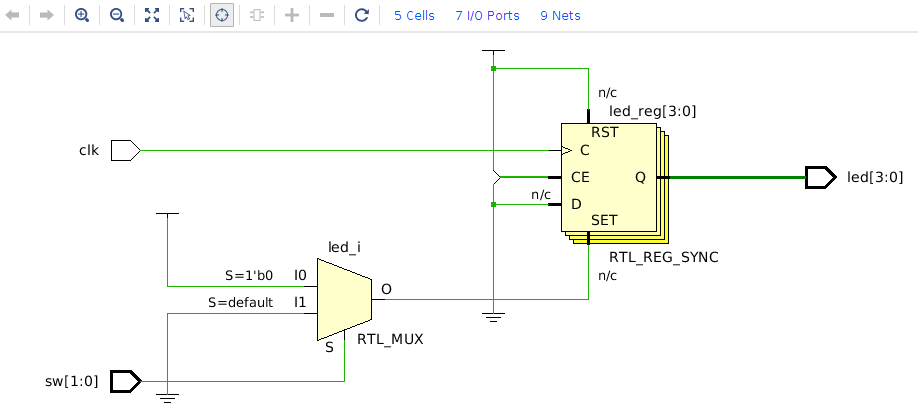
\includegraphics[width=10cm]{S0L0_RTL.png}}
\caption{\label{fig:S0L0RTL} S0L0 RTL schematic; Xilinx Vivado 2017.4}
\end{figure}

    \begin{figure}
\centerline{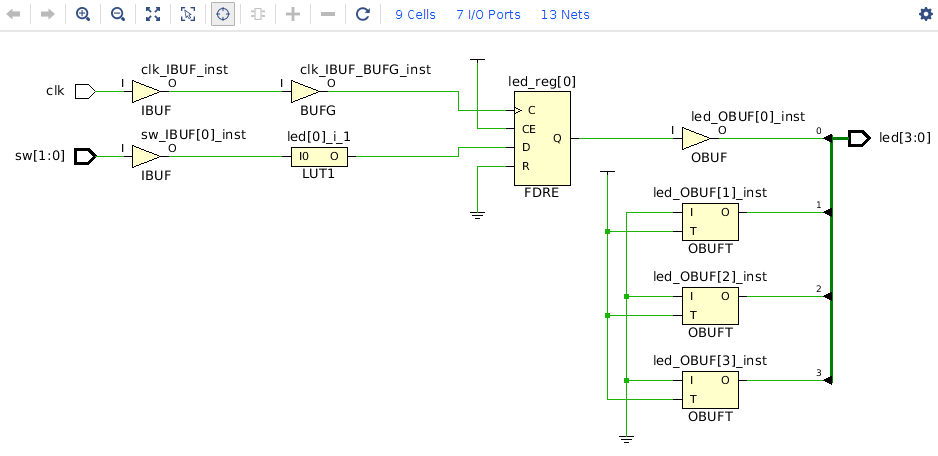
\includegraphics[width=10cm]{S0L0_SYN.png}}
\caption{\label{fig:S0L0SYN} S0L0 Synthesized Schematic; Xilinx Vivado 2017.4}
\end{figure}

    \begin{figure}
\centerline{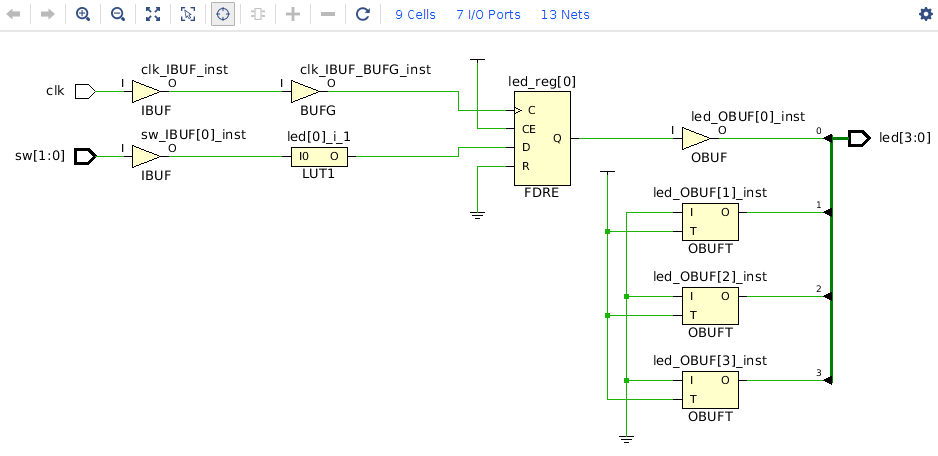
\includegraphics[width=10cm]{S0L0_SYN.png}}
\caption{\label{fig:S0L0SYN} S0L0 Implementated Schematic; Xilinx Vivado 2017.4}
\end{figure}

    \subsection{PYNQ-Z1 Constraints File}\label{pynq-z1-constraints-file}

Below is what is found in file \texttt{constrs\_S0L0.xdc}

Notice that the original port names found in the PYNQ-Z1 Constraints
file have been changed to the port names in the module \texttt{S0L0}
## PYNQ-Z1 Board Constraints for S0L0.v
## Based on https://github.com/Xilinx/PYNQ/blob/master/sdbuild/boot_configs/Pynq-Z1-defconfig/constraints.xdc

## Clock signal 125 MHz

set_property -dict { PACKAGE_PIN H16   IOSTANDARD LVCMOS33 } [get_ports { clk }]; #IO_L13P_T2_MRCC_35 Sch=clk
create_clock -add -name sys_clk_pin -period 8.00 -waveform {0 4} [get_ports { clk }];

## Switches
set_property -dict {PACKAGE_PIN M20 IOSTANDARD LVCMOS33} [get_ports {sw[0]}]
set_property -dict {PACKAGE_PIN M19 IOSTANDARD LVCMOS33} [get_ports {sw[1]}]


##LEDs
set_property -dict {PACKAGE_PIN R14 IOSTANDARD LVCMOS33} [get_ports {led[0]}]
set_property -dict {PACKAGE_PIN P14 IOSTANDARD LVCMOS33} [get_ports {led[1]}]
set_property -dict {PACKAGE_PIN N16 IOSTANDARD LVCMOS33} [get_ports {led[2]}]
set_property -dict {PACKAGE_PIN M14 IOSTANDARD LVCMOS33} [get_ports {led[3]}]
    \subsection{Verilog Testbench}\label{verilog-testbench}

    \begin{Verbatim}[commandchars=\\\{\}]
{\color{incolor}In [{\color{incolor}10}]:} \PY{n}{swTVal}\PY{o}{=}\PY{n}{intbv}\PY{p}{(}\PY{n+nb}{int}\PY{p}{(}\PY{l+s+s1}{\PYZsq{}}\PY{l+s+s1}{\PYZsq{}}\PY{o}{.}\PY{n}{join}\PY{p}{(}\PY{p}{[}\PY{n+nb}{str}\PY{p}{(}\PY{n}{i}\PY{p}{)} \PY{k}{for} \PY{n}{i} \PY{o+ow}{in} \PY{n}{swTVals}\PY{p}{]}\PY{p}{)}\PY{p}{,} \PY{l+m+mi}{2}\PY{p}{)}\PY{p}{)}\PY{p}{[}\PY{n+nb}{len}\PY{p}{(}\PY{n}{swTVals}\PY{p}{)}\PY{p}{:}\PY{p}{]}
         \PY{n+nb}{print}\PY{p}{(}\PY{n}{f}\PY{l+s+s1}{\PYZsq{}}\PY{l+s+s1}{swTest: }\PY{l+s+si}{\PYZob{}swTVals\PYZcb{}}\PY{l+s+s1}{, }\PY{l+s+si}{\PYZob{}swTVal\PYZcb{}}\PY{l+s+s1}{, }\PY{l+s+s1}{\PYZob{}}\PY{l+s+s1}{[int(i) for i in swTVal]\PYZcb{}}\PY{l+s+s1}{\PYZsq{}}\PY{p}{)}
\end{Verbatim}


    \begin{Verbatim}[commandchars=\\\{\}]
swTest: [0, 1, 0, 1, 0, 1, 0, 0, 0, 0], 150, [0, 1, 0, 1, 0, 1, 0, 0, 0, 0]

    \end{Verbatim}

    \begin{Verbatim}[commandchars=\\\{\}]
{\color{incolor}In [{\color{incolor}11}]:} \PY{n+nd}{@block}
         \PY{k}{def} \PY{n+nf}{S0L0\PYZus{}TBV}\PY{p}{(}\PY{p}{)}\PY{p}{:}
             \PY{l+s+sd}{\PYZdq{}\PYZdq{}\PYZdq{}}
         \PY{l+s+sd}{    myHDL \PYZhy{}\PYZgt{} Verilog Testbench for `S0L0`}
         \PY{l+s+sd}{    \PYZdq{}\PYZdq{}\PYZdq{}}
             \PY{n}{clk}\PY{o}{=}\PY{n}{Signal}\PY{p}{(}\PY{n+nb}{bool}\PY{p}{(}\PY{l+m+mi}{0}\PY{p}{)}\PY{p}{)}
             \PY{n}{sw}\PY{o}{=}\PY{n}{Signal}\PY{p}{(}\PY{n}{intbv}\PY{p}{(}\PY{l+m+mi}{0}\PY{p}{)}\PY{p}{[}\PY{l+m+mi}{2}\PY{p}{:}\PY{p}{]}\PY{p}{)}
             \PY{n}{led}\PY{o}{=}\PY{n}{Signal}\PY{p}{(}\PY{n}{intbv}\PY{p}{(}\PY{l+m+mi}{0}\PY{p}{)}\PY{p}{[}\PY{l+m+mi}{4}\PY{p}{:}\PY{p}{]}\PY{p}{)}
             
             \PY{c+c1}{\PYZsh{}test stimuli}
             \PY{n}{swTVals}\PY{o}{=}\PY{n}{Signal}\PY{p}{(}\PY{n}{swTVal}\PY{p}{)}
             
             \PY{n+nd}{@always\PYZus{}comb}
             \PY{k}{def} \PY{n+nf}{print\PYZus{}data}\PY{p}{(}\PY{p}{)}\PY{p}{:}
                 \PY{n+nb}{print}\PY{p}{(}\PY{n}{sw}\PY{p}{,} \PY{n}{clk}\PY{p}{,} \PY{n}{led}\PY{p}{)}
         
         
             \PY{n}{DUT}\PY{o}{=}\PY{n}{S0L0}\PY{p}{(}\PY{n}{sw}\PY{p}{,} \PY{n}{clk}\PY{p}{,} \PY{n}{led}\PY{p}{)}
             
             \PY{n+nd}{@instance}
             \PY{k}{def} \PY{n+nf}{clk\PYZus{}signal}\PY{p}{(}\PY{p}{)}\PY{p}{:}
                 \PY{k}{while} \PY{k+kc}{True}\PY{p}{:}
                     \PY{n}{clk}\PY{o}{.}\PY{n}{next} \PY{o}{=} \PY{o+ow}{not} \PY{n}{clk}
                     \PY{k}{yield} \PY{n}{delay}\PY{p}{(}\PY{l+m+mi}{1}\PY{p}{)}
                 
             \PY{n+nd}{@instance}
             \PY{k}{def} \PY{n+nf}{stimules}\PY{p}{(}\PY{p}{)}\PY{p}{:}
                 \PY{k}{for} \PY{n}{i} \PY{o+ow}{in} \PY{n+nb}{range}\PY{p}{(}\PY{l+m+mi}{10}\PY{p}{)}\PY{p}{:}
                     \PY{n}{sw}\PY{o}{.}\PY{n}{next}\PY{p}{[}\PY{l+m+mi}{0}\PY{p}{]}\PY{o}{=}\PY{n}{swTVals}\PY{p}{[}\PY{n}{i}\PY{p}{]}
                     \PY{k}{yield} \PY{n}{clk}\PY{o}{.}\PY{n}{posedge}
                 \PY{k}{raise} \PY{n}{StopSimulation}\PY{p}{(}\PY{p}{)}
             
             \PY{k}{return} \PY{n}{instances}\PY{p}{(}\PY{p}{)}
                     
         \PY{n}{TB}\PY{o}{=}\PY{n}{S0L0\PYZus{}TBV}\PY{p}{(}\PY{p}{)}
         \PY{n}{TB}\PY{o}{.}\PY{n}{convert}\PY{p}{(}\PY{n}{hdl}\PY{o}{=}\PY{l+s+s2}{\PYZdq{}}\PY{l+s+s2}{Verilog}\PY{l+s+s2}{\PYZdq{}}\PY{p}{,} \PY{n}{initial\PYZus{}values}\PY{o}{=}\PY{k+kc}{True}\PY{p}{)}
         \PY{n}{VerilogTextReader}\PY{p}{(}\PY{l+s+s1}{\PYZsq{}}\PY{l+s+s1}{S0L0\PYZus{}TBV}\PY{l+s+s1}{\PYZsq{}}\PY{p}{)}\PY{p}{;}
\end{Verbatim}


    \begin{Verbatim}[commandchars=\\\{\}]
<class 'myhdl.\_Signal.\_Signal'> <class '\_ast.Name'>
<class 'myhdl.\_Signal.\_Signal'> <class '\_ast.Name'>
<class 'myhdl.\_Signal.\_Signal'> <class '\_ast.Name'>
***Verilog modual from S0L0\_TBV.v***

 // File: S0L0\_TBV.v
// Generated by MyHDL 0.10
// Date: Mon Aug 20 10:39:19 2018


`timescale 1ns/10ps

module S0L0\_TBV (

);
// myHDL -> Verilog Testbench for `S0L0`


reg clk = 0;
reg [1:0] sw = 0;
reg [3:0] led = 0;
wire [9:0] swTVals;

assign swTVals = 10'd336;


always @(sw, led, clk) begin: S0L0\_TBV\_PRINT\_DATA
    \$write("\%h", sw);
    \$write(" ");
    \$write("\%h", clk);
    \$write(" ");
    \$write("\%h", led);
    \$write("\textbackslash{}n");
end


always @(posedge clk) begin: S0L0\_TBV\_S0L00\_0\_LOGIC
    if ((sw[0] == 0)) begin
        led[0] <= 1'b1;
    end
    else begin
        led[0] <= 1'b0;
    end
end


initial begin: S0L0\_TBV\_CLK\_SIGNAL
    while (1'b1) begin
        clk <= (!clk);
        \# 1;
    end
end


initial begin: S0L0\_TBV\_STIMULES
    integer i;
    for (i=0; i<10; i=i+1) begin
        sw[0] <= swTVals[i];
        @(posedge clk);
    end
    \$finish;
end

endmodule


    \end{Verbatim}

    \begin{Verbatim}[commandchars=\\\{\}]
/home/iridium/anaconda3/lib/python3.6/site-packages/myhdl/conversion/\_toVerilog.py:349: ToVerilogWarning: Signal is not driven: swTVals
  category=ToVerilogWarning

    \end{Verbatim}

    \subsection{Board Verification}\label{board-verification}

    \section{Project 2: 2 Switches 4
LEDS}\label{project-2-2-switches-4-leds}

From https://timetoexplore.net/blog/arty-fpga-verilog-01 uses both
Switches on the PYNQ-Z1 to control that on/off states of the four leds
on the PYNQ-Z1

    \subsection{myHDL Code}\label{myhdl-code}

    \begin{Verbatim}[commandchars=\\\{\}]
{\color{incolor}In [{\color{incolor}14}]:} \PY{n+nd}{@block}
         \PY{k}{def} \PY{n+nf}{S2L4}\PY{p}{(}\PY{n}{sw}\PY{p}{,} \PY{n}{clk}\PY{p}{,} \PY{n}{led}\PY{p}{)}\PY{p}{:}
             \PY{l+s+sd}{\PYZdq{}\PYZdq{}\PYZdq{}}
         \PY{l+s+sd}{    FPGA Hello world of two switchs controlling four LEDs based on}
         \PY{l+s+sd}{    https://timetoexplore.net/blog/arty\PYZhy{}fpga\PYZhy{}verilog\PYZhy{}01}
         \PY{l+s+sd}{    }
         \PY{l+s+sd}{    Target:}
         \PY{l+s+sd}{        ZYNQ 7000 Board (Arty, PYNQ\PYZhy{}Z1, PYNQ\PYZhy{}Z2) with at least 2 }
         \PY{l+s+sd}{        switchs and 4 leds}
         \PY{l+s+sd}{    }
         \PY{l+s+sd}{    }
         \PY{l+s+sd}{    Input:}
         \PY{l+s+sd}{        sw(2bitVec):switch input from PYNQ\PYZhy{}Z1/2 (ect.)}
         \PY{l+s+sd}{        clk(bool): clock input    }
         \PY{l+s+sd}{    Ouput:}
         \PY{l+s+sd}{        led(4bitVec): led output to PYNQ\PYZhy{}Z1/2 (ect.)}
         \PY{l+s+sd}{        }
         \PY{l+s+sd}{    \PYZdq{}\PYZdq{}\PYZdq{}}
                 
             \PY{n+nd}{@always}\PY{p}{(}\PY{n}{clk}\PY{o}{.}\PY{n}{posedge}\PY{p}{)}
             \PY{k}{def} \PY{n+nf}{logic}\PY{p}{(}\PY{p}{)}\PY{p}{:}
                 \PY{k}{if} \PY{n}{sw}\PY{p}{[}\PY{l+m+mi}{0}\PY{p}{]}\PY{o}{==}\PY{l+m+mi}{0}\PY{p}{:}
                     \PY{n}{led}\PY{o}{.}\PY{n}{next}\PY{p}{[}\PY{l+m+mi}{2}\PY{p}{:}\PY{p}{]}\PY{o}{=}\PY{l+m+mi}{0}
                 \PY{k}{else}\PY{p}{:}
                     \PY{n}{led}\PY{o}{.}\PY{n}{next}\PY{p}{[}\PY{l+m+mi}{2}\PY{p}{:}\PY{p}{]}\PY{o}{=}\PY{l+m+mi}{3}
                     
                 \PY{k}{if} \PY{n}{sw}\PY{p}{[}\PY{l+m+mi}{1}\PY{p}{]}\PY{o}{==}\PY{l+m+mi}{0}\PY{p}{:}
                     \PY{n}{led}\PY{o}{.}\PY{n}{next}\PY{p}{[}\PY{l+m+mi}{4}\PY{p}{:}\PY{l+m+mi}{2}\PY{p}{]}\PY{o}{=}\PY{l+m+mi}{0}
                 \PY{k}{else}\PY{p}{:}
                     \PY{n}{led}\PY{o}{.}\PY{n}{next}\PY{p}{[}\PY{l+m+mi}{4}\PY{p}{:}\PY{l+m+mi}{2}\PY{p}{]}\PY{o}{=}\PY{l+m+mi}{3}
             
             \PY{k}{return} \PY{n}{instances}\PY{p}{(}\PY{p}{)}
\end{Verbatim}


    \subsection{myHDL Testing}\label{myhdl-testing}

    \begin{Verbatim}[commandchars=\\\{\}]
{\color{incolor}In [{\color{incolor}15}]:} \PY{n}{Peeker}\PY{o}{.}\PY{n}{clear}\PY{p}{(}\PY{p}{)}
         \PY{n}{clk}\PY{o}{=}\PY{n}{Signal}\PY{p}{(}\PY{n+nb}{bool}\PY{p}{(}\PY{l+m+mi}{0}\PY{p}{)}\PY{p}{)}\PY{p}{;} \PY{n}{Peeker}\PY{p}{(}\PY{n}{clk}\PY{p}{,} \PY{l+s+s1}{\PYZsq{}}\PY{l+s+s1}{clk}\PY{l+s+s1}{\PYZsq{}}\PY{p}{)}
         \PY{n}{sw}\PY{o}{=}\PY{n}{Signal}\PY{p}{(}\PY{n}{intbv}\PY{p}{(}\PY{l+m+mi}{0}\PY{p}{)}\PY{p}{[}\PY{l+m+mi}{2}\PY{p}{:}\PY{p}{]}\PY{p}{)}\PY{p}{;} \PY{n}{Peeker}\PY{p}{(}\PY{n}{sw}\PY{p}{,} \PY{l+s+s1}{\PYZsq{}}\PY{l+s+s1}{sw}\PY{l+s+s1}{\PYZsq{}}\PY{p}{)}
         \PY{n}{led}\PY{o}{=}\PY{n}{Signal}\PY{p}{(}\PY{n}{intbv}\PY{p}{(}\PY{l+m+mi}{0}\PY{p}{)}\PY{p}{[}\PY{l+m+mi}{4}\PY{p}{:}\PY{p}{]}\PY{p}{)}\PY{p}{;} \PY{n}{Peeker}\PY{p}{(}\PY{n}{led}\PY{p}{,} \PY{l+s+s1}{\PYZsq{}}\PY{l+s+s1}{led}\PY{l+s+s1}{\PYZsq{}}\PY{p}{)}
         
         \PY{n}{np}\PY{o}{.}\PY{n}{random}\PY{o}{.}\PY{n}{seed}\PY{p}{(}\PY{l+m+mi}{18}\PY{p}{)}
         \PY{n}{swTVals}\PY{o}{=}\PY{p}{[}\PY{n+nb}{int}\PY{p}{(}\PY{n}{i}\PY{p}{)} \PY{k}{for} \PY{n}{i} \PY{o+ow}{in} \PY{n}{np}\PY{o}{.}\PY{n}{random}\PY{o}{.}\PY{n}{randint}\PY{p}{(}\PY{l+m+mi}{0}\PY{p}{,}\PY{l+m+mi}{4}\PY{p}{,} \PY{l+m+mi}{10}\PY{p}{)}\PY{p}{]}
         
         \PY{n}{DUT}\PY{o}{=}\PY{n}{S2L4}\PY{p}{(}\PY{n}{sw}\PY{p}{,} \PY{n}{clk}\PY{p}{,} \PY{n}{led}\PY{p}{)}
         
         \PY{k}{def} \PY{n+nf}{S2L4\PYZus{}TB}\PY{p}{(}\PY{p}{)}\PY{p}{:}
             \PY{l+s+sd}{\PYZdq{}\PYZdq{}\PYZdq{}}
         \PY{l+s+sd}{    myHDL only Testbench for `S2L4`}
         \PY{l+s+sd}{    \PYZdq{}\PYZdq{}\PYZdq{}}
             
             \PY{n+nd}{@always}\PY{p}{(}\PY{n}{delay}\PY{p}{(}\PY{l+m+mi}{1}\PY{p}{)}\PY{p}{)}
             \PY{k}{def} \PY{n+nf}{ClkGen}\PY{p}{(}\PY{p}{)}\PY{p}{:}
                 \PY{n}{clk}\PY{o}{.}\PY{n}{next}\PY{o}{=}\PY{o+ow}{not} \PY{n}{clk}
                 
             \PY{n+nd}{@instance}
             \PY{k}{def} \PY{n+nf}{stimules}\PY{p}{(}\PY{p}{)}\PY{p}{:}
                 \PY{k}{for} \PY{n}{i} \PY{o+ow}{in} \PY{n+nb}{range}\PY{p}{(}\PY{l+m+mi}{10}\PY{p}{)}\PY{p}{:}
                     \PY{n}{sw}\PY{o}{.}\PY{n}{next}\PY{o}{=}\PY{n}{swTVals}\PY{p}{[}\PY{n}{i}\PY{p}{]}
                     \PY{k}{yield} \PY{n}{clk}\PY{o}{.}\PY{n}{posedge}
                 \PY{k}{raise} \PY{n}{StopSimulation}\PY{p}{(}\PY{p}{)}
             
             \PY{k}{return} \PY{n}{instances}\PY{p}{(}\PY{p}{)}
                     
         \PY{n}{sim}\PY{o}{=}\PY{n}{Simulation}\PY{p}{(}\PY{n}{DUT}\PY{p}{,} \PY{n}{S2L4\PYZus{}TB}\PY{p}{(}\PY{p}{)}\PY{p}{,} \PY{o}{*}\PY{n}{Peeker}\PY{o}{.}\PY{n}{instances}\PY{p}{(}\PY{p}{)}\PY{p}{)}\PY{o}{.}\PY{n}{run}\PY{p}{(}\PY{p}{)}
\end{Verbatim}


    \begin{Verbatim}[commandchars=\\\{\}]
{\color{incolor}In [{\color{incolor}16}]:} \PY{n}{Peeker}\PY{o}{.}\PY{n}{to\PYZus{}wavedrom}\PY{p}{(}\PY{p}{)}
\end{Verbatim}


    
    
    
    
    \begin{Verbatim}[commandchars=\\\{\}]
{\color{incolor}In [{\color{incolor}18}]:} \PY{n}{S2L4Data}\PY{o}{=}\PY{n}{Peeker}\PY{o}{.}\PY{n}{to\PYZus{}dataframe}\PY{p}{(}\PY{p}{)}
         \PY{n}{S2L4Data}\PY{o}{=}\PY{n}{S2L4Data}\PY{p}{[}\PY{n}{S2L4Data}\PY{p}{[}\PY{l+s+s1}{\PYZsq{}}\PY{l+s+s1}{clk}\PY{l+s+s1}{\PYZsq{}}\PY{p}{]}\PY{o}{==}\PY{l+m+mi}{1}\PY{p}{]}
         \PY{n}{S2L4Data}\PY{o}{.}\PY{n}{reset\PYZus{}index}\PY{p}{(}\PY{n}{drop}\PY{o}{=}\PY{k+kc}{True}\PY{p}{,} \PY{n}{inplace}\PY{o}{=}\PY{k+kc}{True}\PY{p}{)}
         \PY{n}{S2L4Data}
\end{Verbatim}


\begin{Verbatim}[commandchars=\\\{\}]
{\color{outcolor}Out[{\color{outcolor}18}]:}    clk  led  sw
         0    1   12   3
         1    1   15   0
         2    1    0   1
         3    1    3   2
         4    1   12   1
         5    1    3   2
         6    1   12   2
         7    1   12   2
         8    1   12   0
\end{Verbatim}
            
    \subsection{Verilog Code}\label{verilog-code}

    \begin{Verbatim}[commandchars=\\\{\}]
{\color{incolor}In [{\color{incolor}19}]:} \PY{n}{DUT}\PY{o}{.}\PY{n}{convert}\PY{p}{(}\PY{p}{)}
         \PY{n}{VerilogTextReader}\PY{p}{(}\PY{l+s+s1}{\PYZsq{}}\PY{l+s+s1}{S2L4}\PY{l+s+s1}{\PYZsq{}}\PY{p}{)}\PY{p}{;}
\end{Verbatim}


    \begin{Verbatim}[commandchars=\\\{\}]
***Verilog modual from S2L4.v***

 // File: S2L4.v
// Generated by MyHDL 0.10
// Date: Mon Aug 20 10:46:58 2018


`timescale 1ns/10ps

module S2L4 (
    sw,
    clk,
    led
);
// FPGA Hello world of one switch controlling one LED based on
// https://timetoexplore.net/blog/arty-fpga-verilog-01
// 
// Target:
//     ZYNQ 7000 Board (Arty, PYNQ-Z1, PYNQ-Z2) with at least 2 
//     switchs and 4 leds
// 
// 
// Input:
//     sw(2bitVec):switch input from PYNQ-Z1/2 (ect.)
//     clk(bool): clock input    
// Ouput:
//     led(4bitVec): led output to PYNQ-Z1/2 (ect.)
//     

input [1:0] sw;
input clk;
output [3:0] led;
reg [3:0] led;




always @(posedge clk) begin: S2L4\_LOGIC
    if ((sw[0] == 0)) begin
        led[2-1:0] <= 0;
    end
    else begin
        led[2-1:0] <= 3;
    end
    if ((sw[1] == 0)) begin
        led[4-1:2] <= 0;
    end
    else begin
        led[4-1:2] <= 3;
    end
end

endmodule


    \end{Verbatim}

    \begin{figure}
\centerline{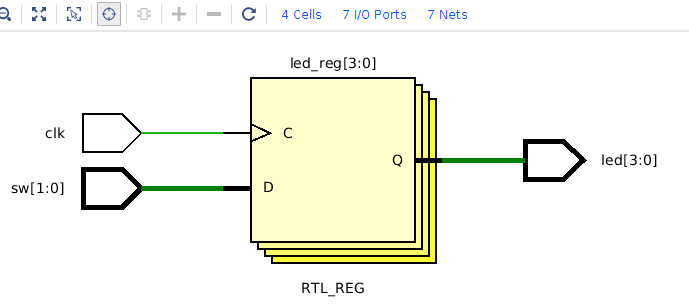
\includegraphics[width=10cm]{S2L4_RTL.png}}
\caption{\label{fig:S2L4RTL} S2L4 RTL schematic; Xilinx Vivado 2017.4}
\end{figure}

    \begin{figure}
\centerline{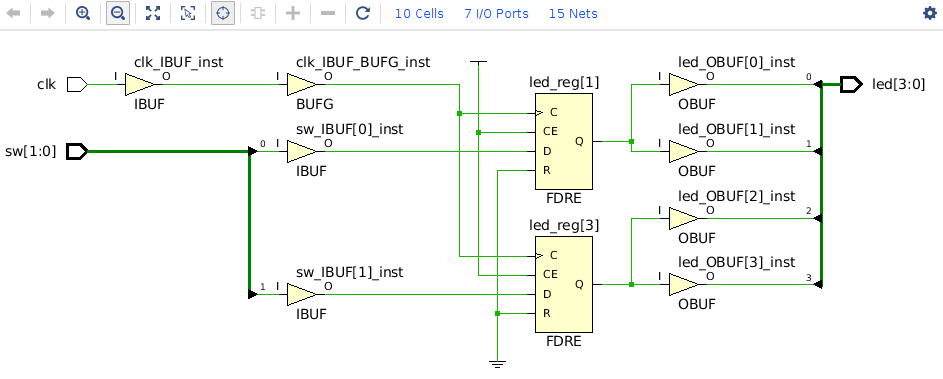
\includegraphics[width=10cm]{S2L4_SYN.png}}
\caption{\label{fig:S2L4SYN} S2L4 Synthesized Schematic; Xilinx Vivado 2017.4}
\end{figure}

    \begin{figure}
\centerline{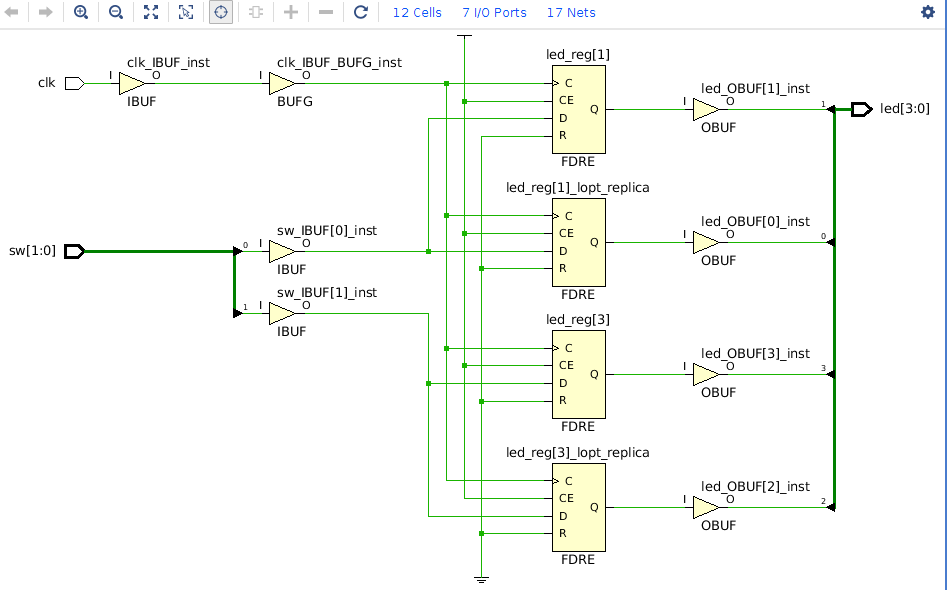
\includegraphics[width=10cm]{S2L4_IMP.png}}
\caption{\label{fig:S2L4SYN} S2L4 Implementated Schematic; Xilinx Vivado 2017.4}
\end{figure}

    \subsection{Verilog Testbench (ToDo)}\label{verilog-testbench-todo}

will write later when testbench conversion is improved

    \subsection{PYNQ-Z1 Constraints File}\label{pynq-z1-constraints-file}

using same one as in \textbf{Project 1: 1 Switch 1 LED}:
\texttt{constrs\_S0L0.xdc}

    \subsection{Board Verification}\label{board-verification}

    \section{Project 3: Countdown}\label{project-3-countdown}

From https://timetoexplore.net/blog/arty-fpga-verilog-02 utilizes a
counter that each led samples the bits at different locations to create
various rate pulsed leds

    \subsection{myHDL Code}\label{myhdl-code}

    \begin{Verbatim}[commandchars=\\\{\}]
{\color{incolor}In [{\color{incolor}20}]:} \PY{n+nd}{@block}
         \PY{k}{def} \PY{n+nf}{countLED}\PY{p}{(}\PY{n}{clk}\PY{p}{,} \PY{n}{led}\PY{p}{)}\PY{p}{:}
             \PY{l+s+sd}{\PYZdq{}\PYZdq{}\PYZdq{}}
         \PY{l+s+sd}{    FPGA Hello world of counter sampled led pulsing from}
         \PY{l+s+sd}{    https://timetoexplore.net/blog/arty\PYZhy{}fpga\PYZhy{}verilog\PYZhy{}02}
         \PY{l+s+sd}{    }
         \PY{l+s+sd}{    Target:}
         \PY{l+s+sd}{        ZYNQ 7000 Board (Arty, PYNQ\PYZhy{}Z1, PYNQ\PYZhy{}Z2) with at least 2 }
         \PY{l+s+sd}{        switchs and 4 leds}
         \PY{l+s+sd}{    }
         \PY{l+s+sd}{    }
         \PY{l+s+sd}{    Input:}
         \PY{l+s+sd}{        clk(bool): clock input    }
         \PY{l+s+sd}{    Ouput:}
         \PY{l+s+sd}{        led(4bitVec): led output to PYNQ\PYZhy{}Z1/2 (ect.)}
         \PY{l+s+sd}{        }
         \PY{l+s+sd}{    \PYZdq{}\PYZdq{}\PYZdq{}}
             \PY{n}{counter}\PY{o}{=}\PY{n}{Signal}\PY{p}{(}\PY{n}{modbv}\PY{p}{(}\PY{l+m+mi}{0}\PY{p}{)}\PY{p}{[}\PY{l+m+mi}{33}\PY{p}{:}\PY{p}{]}\PY{p}{)}
             
             \PY{n+nd}{@always}\PY{p}{(}\PY{n}{clk}\PY{o}{.}\PY{n}{posedge}\PY{p}{)}
             \PY{k}{def} \PY{n+nf}{logic}\PY{p}{(}\PY{p}{)}\PY{p}{:}
                 \PY{n}{counter}\PY{o}{.}\PY{n}{next}\PY{o}{=}\PY{n}{counter}\PY{o}{+}\PY{l+m+mi}{1}
                 \PY{n}{led}\PY{o}{.}\PY{n}{next}\PY{p}{[}\PY{l+m+mi}{0}\PY{p}{]}\PY{o}{=}\PY{n}{counter}\PY{p}{[}\PY{l+m+mi}{26}\PY{p}{]}
                 \PY{n}{led}\PY{o}{.}\PY{n}{next}\PY{p}{[}\PY{l+m+mi}{1}\PY{p}{]}\PY{o}{=}\PY{n}{counter}\PY{p}{[}\PY{l+m+mi}{24}\PY{p}{]}
                 \PY{n}{led}\PY{o}{.}\PY{n}{next}\PY{p}{[}\PY{l+m+mi}{2}\PY{p}{]}\PY{o}{=}\PY{n}{counter}\PY{p}{[}\PY{l+m+mi}{22}\PY{p}{]}
                 \PY{n}{led}\PY{o}{.}\PY{n}{next}\PY{p}{[}\PY{l+m+mi}{3}\PY{p}{]}\PY{o}{=}\PY{n}{counter}\PY{p}{[}\PY{l+m+mi}{20}\PY{p}{]}
             
             \PY{k}{return} \PY{n}{instances}\PY{p}{(}\PY{p}{)}
\end{Verbatim}


    \subsection{myHDL Testing (Needs
Improvements)}\label{myhdl-testing-needs-improvements}

    \begin{Verbatim}[commandchars=\\\{\}]
{\color{incolor}In [{\color{incolor}22}]:} \PY{n}{Peeker}\PY{o}{.}\PY{n}{clear}\PY{p}{(}\PY{p}{)}
         \PY{n}{clk}\PY{o}{=}\PY{n}{Signal}\PY{p}{(}\PY{n+nb}{bool}\PY{p}{(}\PY{l+m+mi}{0}\PY{p}{)}\PY{p}{)}\PY{p}{;} \PY{n}{Peeker}\PY{p}{(}\PY{n}{clk}\PY{p}{,} \PY{l+s+s1}{\PYZsq{}}\PY{l+s+s1}{clk}\PY{l+s+s1}{\PYZsq{}}\PY{p}{)}
         \PY{n}{led}\PY{o}{=}\PY{n}{Signal}\PY{p}{(}\PY{n}{intbv}\PY{p}{(}\PY{l+m+mi}{0}\PY{p}{)}\PY{p}{[}\PY{l+m+mi}{4}\PY{p}{:}\PY{p}{]}\PY{p}{)}\PY{p}{;} \PY{n}{Peeker}\PY{p}{(}\PY{n}{led}\PY{p}{,} \PY{l+s+s1}{\PYZsq{}}\PY{l+s+s1}{led}\PY{l+s+s1}{\PYZsq{}}\PY{p}{)}
         
         
         \PY{n}{DUT}\PY{o}{=}\PY{n}{countLED}\PY{p}{(}\PY{n}{clk}\PY{p}{,} \PY{n}{led}\PY{p}{)}
         
         \PY{c+c1}{\PYZsh{}testbench it too slow as it}
         \PY{l+s+sd}{\PYZsq{}\PYZsq{}\PYZsq{}}
         \PY{l+s+sd}{def countLED\PYZus{}TB():}
         \PY{l+s+sd}{    \PYZdq{}\PYZdq{}\PYZdq{}}
         \PY{l+s+sd}{    myHDL only Testbench for `countLED`}
         \PY{l+s+sd}{    \PYZdq{}\PYZdq{}\PYZdq{}}
         \PY{l+s+sd}{    }
         \PY{l+s+sd}{    @always(delay(1))}
         \PY{l+s+sd}{    def ClkGen():}
         \PY{l+s+sd}{        clk.next=not clk}
         \PY{l+s+sd}{        }
         \PY{l+s+sd}{    @instance}
         \PY{l+s+sd}{    def stimules():}
         \PY{l+s+sd}{        i=0}
         \PY{l+s+sd}{        while True:}
         \PY{l+s+sd}{            if i==2**33:}
         \PY{l+s+sd}{                raise StopSimulation()}
         \PY{l+s+sd}{            if 1\PYZpc{}100==0:}
         \PY{l+s+sd}{                print(i)}
         \PY{l+s+sd}{            i+=1}
         \PY{l+s+sd}{            yield clk.posedge}
         \PY{l+s+sd}{    }
         \PY{l+s+sd}{    return instances()}
         \PY{l+s+sd}{            }
         \PY{l+s+sd}{sim=Simulation(DUT, countLED\PYZus{}TB(), *Peeker.instances()).run()}
         \PY{l+s+sd}{\PYZsq{}\PYZsq{}\PYZsq{}}
         \PY{p}{;}
\end{Verbatim}


\begin{Verbatim}[commandchars=\\\{\}]
{\color{outcolor}Out[{\color{outcolor}22}]:} ''
\end{Verbatim}
            
    Need to figure out how to write/run these long simulations better in
python

    \subsection{Verilog Code}\label{verilog-code}

    \begin{Verbatim}[commandchars=\\\{\}]
{\color{incolor}In [{\color{incolor}23}]:} \PY{n}{DUT}\PY{o}{.}\PY{n}{convert}\PY{p}{(}\PY{p}{)}
         \PY{n}{VerilogTextReader}\PY{p}{(}\PY{l+s+s1}{\PYZsq{}}\PY{l+s+s1}{countLED}\PY{l+s+s1}{\PYZsq{}}\PY{p}{)}\PY{p}{;}
\end{Verbatim}


    \begin{Verbatim}[commandchars=\\\{\}]
***Verilog modual from countLED.v***

 // File: countLED.v
// Generated by MyHDL 0.10
// Date: Mon Aug 20 10:53:10 2018


`timescale 1ns/10ps

module countLED (
    clk,
    led
);
// FPGA Hello world of counter sampled led pulsing from
// https://timetoexplore.net/blog/arty-fpga-verilog-02
// 
// Target:
//     ZYNQ 7000 Board (Arty, PYNQ-Z1, PYNQ-Z2) with at least 2 
//     switchs and 4 leds
// 
// 
// Input:
//     clk(bool): clock input    
// Ouput:
//     led(4bitVec): led output to PYNQ-Z1/2 (ect.)
//     

input clk;
output [3:0] led;
reg [3:0] led;

reg [32:0] counter = 0;



always @(posedge clk) begin: COUNTLED\_LOGIC
    counter <= (counter + 1);
    led[0] <= counter[26];
    led[1] <= counter[24];
    led[2] <= counter[22];
    led[3] <= counter[20];
end

endmodule


    \end{Verbatim}

    \begin{figure}
\centerline{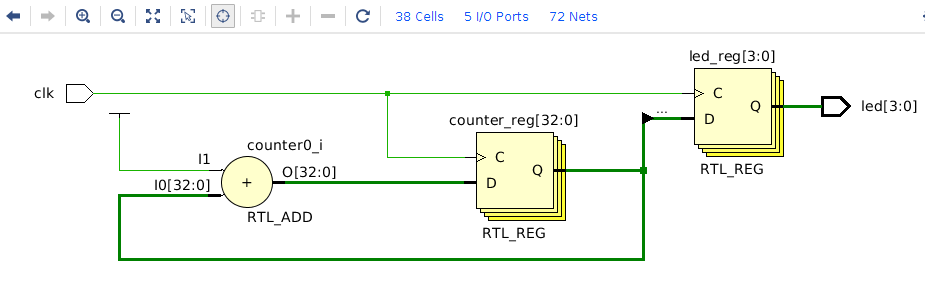
\includegraphics[width=10cm]{countLEDRTL.png}}
\caption{\label{fig:countLEDRTL} countLED RTL schematic; Xilinx Vivado 2017.4}
\end{figure}

    \begin{figure}
\centerline{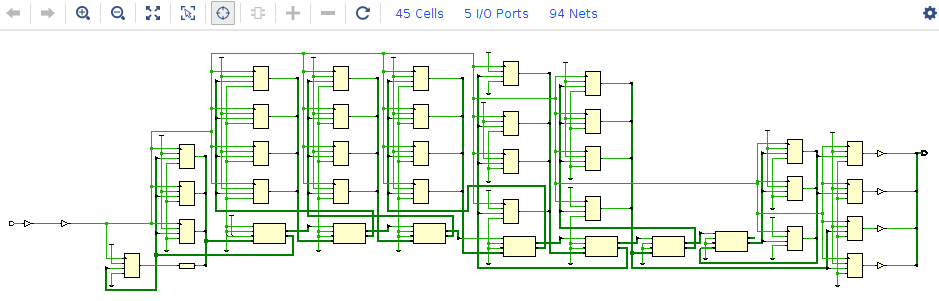
\includegraphics[width=10cm]{countLEDSYN.png}}
\caption{\label{fig:countLEDSYN} countLED Synthesized Schematic; Xilinx Vivado 2017.4}
\end{figure}

    \begin{figure}
\centerline{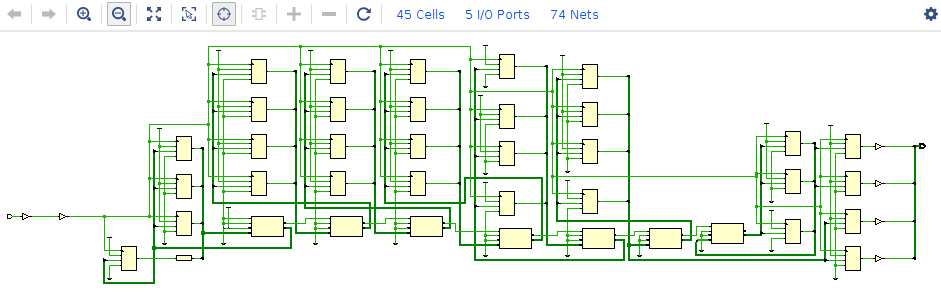
\includegraphics[width=10cm]{countLEDIMP.png}}
\caption{\label{fig:countLEDSYN} countLED Implementated Schematic; Xilinx Vivado 2017.4}
\end{figure}

    \subsection{Verilog Testbench}\label{verilog-testbench}

    \subsubsection{Conversion Issue}\label{conversion-issue}

\texttt{2**33} was converted literally to \texttt{2**33} in the
resulting Verilog code instead of \texttt{8589934592} as it should have
been

    \begin{Verbatim}[commandchars=\\\{\}]
{\color{incolor}In [{\color{incolor}24}]:} \PY{n+nd}{@block}
         \PY{k}{def} \PY{n+nf}{countLED\PYZus{}TBV}\PY{p}{(}\PY{p}{)}\PY{p}{:}
             \PY{l+s+sd}{\PYZdq{}\PYZdq{}\PYZdq{}}
         \PY{l+s+sd}{    myHDL \PYZhy{}\PYZgt{} Verilog Testbench for `countLED`}
         \PY{l+s+sd}{    Note:}
         \PY{l+s+sd}{        Need to improve this testbench}
         \PY{l+s+sd}{    \PYZdq{}\PYZdq{}\PYZdq{}}
             \PY{n}{clk}\PY{o}{=}\PY{n}{Signal}\PY{p}{(}\PY{n+nb}{bool}\PY{p}{(}\PY{l+m+mi}{0}\PY{p}{)}\PY{p}{)}
             \PY{n}{led}\PY{o}{=}\PY{n}{Signal}\PY{p}{(}\PY{n}{intbv}\PY{p}{(}\PY{l+m+mi}{0}\PY{p}{)}\PY{p}{[}\PY{l+m+mi}{4}\PY{p}{:}\PY{p}{]}\PY{p}{)}
             
             \PY{n+nd}{@always\PYZus{}comb}
             \PY{k}{def} \PY{n+nf}{print\PYZus{}data}\PY{p}{(}\PY{p}{)}\PY{p}{:}
                 \PY{n+nb}{print}\PY{p}{(}\PY{n}{clk}\PY{p}{,} \PY{n}{led}\PY{p}{)}
         
             \PY{n}{DUT}\PY{o}{=}\PY{n}{countLED}\PY{p}{(}\PY{n}{clk}\PY{p}{,} \PY{n}{led}\PY{p}{)}
         
             \PY{n+nd}{@instance}
             \PY{k}{def} \PY{n+nf}{clk\PYZus{}signal}\PY{p}{(}\PY{p}{)}\PY{p}{:}
                 \PY{k}{while} \PY{k+kc}{True}\PY{p}{:}
                     \PY{n}{clk}\PY{o}{.}\PY{n}{next} \PY{o}{=} \PY{o+ow}{not} \PY{n}{clk}
                     \PY{k}{yield} \PY{n}{delay}\PY{p}{(}\PY{l+m+mi}{1}\PY{p}{)}
            
                 
             \PY{n+nd}{@instance}
             \PY{k}{def} \PY{n+nf}{stimules}\PY{p}{(}\PY{p}{)}\PY{p}{:}
                 \PY{n}{i}\PY{o}{=}\PY{l+m+mi}{0}
                 \PY{k}{while} \PY{k+kc}{True}\PY{p}{:}
                     \PY{k}{if} \PY{n}{i}\PY{o}{==}\PY{l+m+mi}{8589934592}\PY{p}{:}
                         \PY{k}{raise} \PY{n}{StopSimulation}\PY{p}{(}\PY{p}{)}
                     
                     \PY{n}{i}\PY{o}{+}\PY{o}{=}\PY{l+m+mi}{1}
                     \PY{k}{yield} \PY{n}{clk}\PY{o}{.}\PY{n}{posedge}
             
             \PY{k}{return} \PY{n}{instances}\PY{p}{(}\PY{p}{)}
                     
         \PY{n}{TB}\PY{o}{=}\PY{n}{countLED\PYZus{}TBV}\PY{p}{(}\PY{p}{)}
         \PY{n}{TB}\PY{o}{.}\PY{n}{convert}\PY{p}{(}\PY{n}{hdl}\PY{o}{=}\PY{l+s+s2}{\PYZdq{}}\PY{l+s+s2}{Verilog}\PY{l+s+s2}{\PYZdq{}}\PY{p}{,} \PY{n}{initial\PYZus{}values}\PY{o}{=}\PY{k+kc}{True}\PY{p}{)}
         \PY{n}{VerilogTextReader}\PY{p}{(}\PY{l+s+s1}{\PYZsq{}}\PY{l+s+s1}{countLED\PYZus{}TBV}\PY{l+s+s1}{\PYZsq{}}\PY{p}{)}\PY{p}{;}
\end{Verbatim}


    \begin{Verbatim}[commandchars=\\\{\}]
<class 'myhdl.\_Signal.\_Signal'> <class '\_ast.Name'>
<class 'myhdl.\_Signal.\_Signal'> <class '\_ast.Name'>
***Verilog modual from countLED\_TBV.v***

 // File: countLED\_TBV.v
// Generated by MyHDL 0.10
// Date: Mon Aug 20 10:54:41 2018


`timescale 1ns/10ps

module countLED\_TBV (

);
// myHDL -> Verilog Testbench for `countLED`
// Note:
//     Need to improve this testbench


reg clk = 0;
reg [3:0] led = 0;
reg [32:0] countLED0\_0\_counter = 0;



always @(led, clk) begin: COUNTLED\_TBV\_PRINT\_DATA
    \$write("\%h", clk);
    \$write(" ");
    \$write("\%h", led);
    \$write("\textbackslash{}n");
end


always @(posedge clk) begin: COUNTLED\_TBV\_COUNTLED0\_0\_LOGIC
    countLED0\_0\_counter <= (countLED0\_0\_counter + 1);
    led[0] <= countLED0\_0\_counter[26];
    led[1] <= countLED0\_0\_counter[24];
    led[2] <= countLED0\_0\_counter[22];
    led[3] <= countLED0\_0\_counter[20];
end


initial begin: COUNTLED\_TBV\_CLK\_SIGNAL
    while (1'b1) begin
        clk <= (!clk);
        \# 1;
    end
end


initial begin: COUNTLED\_TBV\_STIMULES
    integer i;
    i = 0;
    while (1'b1) begin
        if ((i == 35'h200000000)) begin
            \$finish;
        end
        i = i + 1;
        @(posedge clk);
    end
end

endmodule


    \end{Verbatim}

    \subsection{PYNQ-Z1 Constraints File}\label{pynq-z1-constraints-file}

Below is what is found in file \texttt{constrs\_countLED.xdc}

Notice that the original port names found in the PYNQ-Z1 Constraints
file have been changed to the port names in the module \texttt{countLED}
## PYNQ-Z1 Board Constraints for countLED.v
## Based on https://github.com/Xilinx/PYNQ/blob/master/sdbuild/boot_configs/Pynq-Z1-defconfig/constraints.xdc

## Clock signal 125 MHz

set_property -dict { PACKAGE_PIN H16   IOSTANDARD LVCMOS33 } [get_ports { clk }]; #IO_L13P_T2_MRCC_35 Sch=clk
create_clock -add -name sys_clk_pin -period 10.00 -waveform {0 5} [get_ports { clk }];



##LEDs
set_property -dict {PACKAGE_PIN R14 IOSTANDARD LVCMOS33} [get_ports {led[0]}]
set_property -dict {PACKAGE_PIN P14 IOSTANDARD LVCMOS33} [get_ports {led[1]}]
set_property -dict {PACKAGE_PIN N16 IOSTANDARD LVCMOS33} [get_ports {led[2]}]
set_property -dict {PACKAGE_PIN M14 IOSTANDARD LVCMOS33} [get_ports {led[3]}]
    \subsection{Board Verification}\label{board-verification}

    \section{Project 4: Basic Duty Cycle}\label{project-4-basic-duty-cycle}

From https://timetoexplore.net/blog/arty-fpga-verilog-02 , this example
utilizes the basic duty cycle on/off from an internal counter to dim the
LEDs

    \subsection{myHDL Code}\label{myhdl-code}

    \begin{Verbatim}[commandchars=\\\{\}]
{\color{incolor}In [{\color{incolor}25}]:} \PY{n+nd}{@block}
         \PY{k}{def} \PY{n+nf}{BDCLed}\PY{p}{(}\PY{n}{clk}\PY{p}{,} \PY{n}{led}\PY{p}{)}\PY{p}{:}
             \PY{l+s+sd}{\PYZdq{}\PYZdq{}\PYZdq{}}
         \PY{l+s+sd}{    FPGA Hello world of counter duty cycle led brightness control}
         \PY{l+s+sd}{    https://timetoexplore.net/blog/arty\PYZhy{}fpga\PYZhy{}verilog\PYZhy{}02}
         \PY{l+s+sd}{    }
         \PY{l+s+sd}{    Target:}
         \PY{l+s+sd}{        ZYNQ 7000 Board (Arty, PYNQ\PYZhy{}Z1, PYNQ\PYZhy{}Z2) with at least 4 leds}
         \PY{l+s+sd}{    }
         \PY{l+s+sd}{    }
         \PY{l+s+sd}{    Input:}
         \PY{l+s+sd}{        clk(bool): clock input    }
         \PY{l+s+sd}{    Ouput:}
         \PY{l+s+sd}{        led(4bitVec): led output to PYNQ\PYZhy{}Z1/2 (ect.)}
         \PY{l+s+sd}{        }
         \PY{l+s+sd}{    \PYZdq{}\PYZdq{}\PYZdq{}}
             \PY{n}{counter}\PY{o}{=}\PY{n}{Signal}\PY{p}{(}\PY{n}{modbv}\PY{p}{(}\PY{l+m+mi}{0}\PY{p}{)}\PY{p}{[}\PY{l+m+mi}{8}\PY{p}{:}\PY{p}{]}\PY{p}{)}
             \PY{n}{duty\PYZus{}led}\PY{o}{=}\PY{n}{Signal}\PY{p}{(}\PY{n}{modbv}\PY{p}{(}\PY{l+m+mi}{8}\PY{p}{)}\PY{p}{[}\PY{l+m+mi}{8}\PY{p}{:}\PY{p}{]}\PY{p}{)}
             
             \PY{n+nd}{@always}\PY{p}{(}\PY{n}{clk}\PY{o}{.}\PY{n}{posedge}\PY{p}{)}
             \PY{k}{def} \PY{n+nf}{logic}\PY{p}{(}\PY{p}{)}\PY{p}{:}
                 \PY{n}{counter}\PY{o}{.}\PY{n}{next}\PY{o}{=}\PY{n}{counter}\PY{o}{+}\PY{l+m+mi}{1}
                 \PY{k}{if} \PY{n}{counter}\PY{o}{\PYZlt{}}\PY{n}{duty\PYZus{}led}\PY{p}{:}
                     \PY{n}{led}\PY{o}{.}\PY{n}{next}\PY{o}{=}\PY{l+m+mi}{15}
                 \PY{k}{else}\PY{p}{:}
                     \PY{n}{led}\PY{o}{.}\PY{n}{next}\PY{o}{=}\PY{l+m+mi}{0}
             
             \PY{k}{return} \PY{n}{instances}\PY{p}{(}\PY{p}{)}
\end{Verbatim}


    \subsection{myHDL Testing}\label{myhdl-testing}

    \begin{Verbatim}[commandchars=\\\{\}]
{\color{incolor}In [{\color{incolor}26}]:} \PY{n}{Peeker}\PY{o}{.}\PY{n}{clear}\PY{p}{(}\PY{p}{)}
         \PY{n}{clk}\PY{o}{=}\PY{n}{Signal}\PY{p}{(}\PY{n+nb}{bool}\PY{p}{(}\PY{l+m+mi}{0}\PY{p}{)}\PY{p}{)}\PY{p}{;} \PY{n}{Peeker}\PY{p}{(}\PY{n}{clk}\PY{p}{,} \PY{l+s+s1}{\PYZsq{}}\PY{l+s+s1}{clk}\PY{l+s+s1}{\PYZsq{}}\PY{p}{)}
         \PY{n}{led}\PY{o}{=}\PY{n}{Signal}\PY{p}{(}\PY{n}{intbv}\PY{p}{(}\PY{l+m+mi}{0}\PY{p}{)}\PY{p}{[}\PY{l+m+mi}{4}\PY{p}{:}\PY{p}{]}\PY{p}{)}\PY{p}{;} \PY{n}{Peeker}\PY{p}{(}\PY{n}{led}\PY{p}{,} \PY{l+s+s1}{\PYZsq{}}\PY{l+s+s1}{led}\PY{l+s+s1}{\PYZsq{}}\PY{p}{)}
         
         \PY{n}{DUT}\PY{o}{=}\PY{n}{BDCLed}\PY{p}{(}\PY{n}{clk}\PY{p}{,} \PY{n}{led}\PY{p}{)}
             
         \PY{k}{def} \PY{n+nf}{BDCLed\PYZus{}TB}\PY{p}{(}\PY{p}{)}\PY{p}{:}
             \PY{l+s+sd}{\PYZdq{}\PYZdq{}\PYZdq{}}
         \PY{l+s+sd}{    myHDL only Testbench for `BDCLed`}
         \PY{l+s+sd}{    \PYZdq{}\PYZdq{}\PYZdq{}}
             
             \PY{n+nd}{@always}\PY{p}{(}\PY{n}{delay}\PY{p}{(}\PY{l+m+mi}{1}\PY{p}{)}\PY{p}{)}
             \PY{k}{def} \PY{n+nf}{ClkGen}\PY{p}{(}\PY{p}{)}\PY{p}{:}
                 \PY{n}{clk}\PY{o}{.}\PY{n}{next}\PY{o}{=}\PY{o+ow}{not} \PY{n}{clk}
                 
             \PY{n+nd}{@instance}
             \PY{k}{def} \PY{n+nf}{stimules}\PY{p}{(}\PY{p}{)}\PY{p}{:}
                 \PY{n}{i}\PY{o}{=}\PY{l+m+mi}{0}
                 \PY{k}{while} \PY{k+kc}{True}\PY{p}{:}
                     \PY{k}{if} \PY{n}{i}\PY{o}{==}\PY{l+m+mi}{1000}\PY{p}{:}
                         \PY{k}{raise} \PY{n}{StopSimulation}\PY{p}{(}\PY{p}{)}
                     \PY{n}{i}\PY{o}{+}\PY{o}{=}\PY{l+m+mi}{1}
                     \PY{k}{yield} \PY{n}{clk}\PY{o}{.}\PY{n}{posedge}
             
             \PY{k}{return} \PY{n}{instances}\PY{p}{(}\PY{p}{)}
                     
         \PY{n}{sim}\PY{o}{=}\PY{n}{Simulation}\PY{p}{(}\PY{n}{DUT}\PY{p}{,} \PY{n}{BDCLed\PYZus{}TB}\PY{p}{(}\PY{p}{)}\PY{p}{,} \PY{o}{*}\PY{n}{Peeker}\PY{o}{.}\PY{n}{instances}\PY{p}{(}\PY{p}{)}\PY{p}{)}\PY{o}{.}\PY{n}{run}\PY{p}{(}\PY{p}{)}
\end{Verbatim}


    \begin{Verbatim}[commandchars=\\\{\}]
{\color{incolor}In [{\color{incolor}27}]:} \PY{n}{Peeker}\PY{o}{.}\PY{n}{to\PYZus{}wavedrom}\PY{p}{(}\PY{p}{)}
\end{Verbatim}


    
    
    
    
    \begin{Verbatim}[commandchars=\\\{\}]
{\color{incolor}In [{\color{incolor}29}]:} \PY{n}{BDCLedData}\PY{o}{=}\PY{n}{Peeker}\PY{o}{.}\PY{n}{to\PYZus{}dataframe}\PY{p}{(}\PY{p}{)}
         \PY{n}{BDCLedData}\PY{o}{=}\PY{n}{BDCLedData}\PY{p}{[}\PY{n}{BDCLedData}\PY{p}{[}\PY{l+s+s1}{\PYZsq{}}\PY{l+s+s1}{clk}\PY{l+s+s1}{\PYZsq{}}\PY{p}{]}\PY{o}{==}\PY{l+m+mi}{1}\PY{p}{]}
         \PY{n}{BDCLedData}\PY{o}{.}\PY{n}{reset\PYZus{}index}\PY{p}{(}\PY{n}{drop}\PY{o}{=}\PY{k+kc}{True}\PY{p}{,} \PY{n}{inplace}\PY{o}{=}\PY{k+kc}{True}\PY{p}{)}
         \PY{n}{BDCLedData}\PY{o}{.}\PY{n}{plot}\PY{p}{(}\PY{n}{y}\PY{o}{=}\PY{l+s+s1}{\PYZsq{}}\PY{l+s+s1}{led}\PY{l+s+s1}{\PYZsq{}}\PY{p}{,} \PY{n}{title}\PY{o}{=}\PY{l+s+s1}{\PYZsq{}}\PY{l+s+s1}{led cycle on time}\PY{l+s+s1}{\PYZsq{}}\PY{p}{)}\PY{p}{;}
\end{Verbatim}


    \begin{center}
    \adjustimage{max size={0.9\linewidth}{0.9\paperheight}}{output_62_0.png}
    \end{center}
    { \hspace*{\fill} \\}
    
    \subsection{Verilog Code}\label{verilog-code}

    \begin{Verbatim}[commandchars=\\\{\}]
{\color{incolor}In [{\color{incolor}30}]:} \PY{n}{DUT}\PY{o}{.}\PY{n}{convert}\PY{p}{(}\PY{p}{)}
         \PY{n}{VerilogTextReader}\PY{p}{(}\PY{l+s+s1}{\PYZsq{}}\PY{l+s+s1}{BDCLed}\PY{l+s+s1}{\PYZsq{}}\PY{p}{)}\PY{p}{;}
\end{Verbatim}


    \begin{Verbatim}[commandchars=\\\{\}]
***Verilog modual from BDCLed.v***

 // File: BDCLed.v
// Generated by MyHDL 0.10
// Date: Mon Aug 20 11:01:43 2018


`timescale 1ns/10ps

module BDCLed (
    clk,
    led
);
// FPGA Hello world of counter duty cycle led brightness control
// https://timetoexplore.net/blog/arty-fpga-verilog-02
// 
// Target:
//     ZYNQ 7000 Board (Arty, PYNQ-Z1, PYNQ-Z2) with at least 4 leds
// 
// 
// Input:
//     clk(bool): clock input    
// Ouput:
//     led(4bitVec): led output to PYNQ-Z1/2 (ect.)
//     

input clk;
output [3:0] led;
reg [3:0] led;

wire [7:0] duty\_led;
reg [7:0] counter = 0;

assign duty\_led = 8'd8;


always @(posedge clk) begin: BDCLED\_LOGIC
    counter <= (counter + 1);
    if ((counter < duty\_led)) begin
        led <= 15;
    end
    else begin
        led <= 0;
    end
end

endmodule


    \end{Verbatim}

    \begin{Verbatim}[commandchars=\\\{\}]
/home/iridium/anaconda3/lib/python3.6/site-packages/myhdl/conversion/\_toVerilog.py:349: ToVerilogWarning: Signal is not driven: duty\_led
  category=ToVerilogWarning

    \end{Verbatim}

    \begin{figure}
\centerline{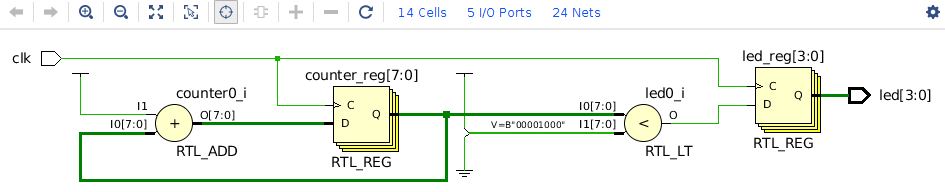
\includegraphics[width=10cm]{BDCLed_RTL.png}}
\caption{\label{fig:BDCLedRTL} BDCLed RTL schematic; Xilinx Vivado 2017.4}
\end{figure}

    \begin{figure}
\centerline{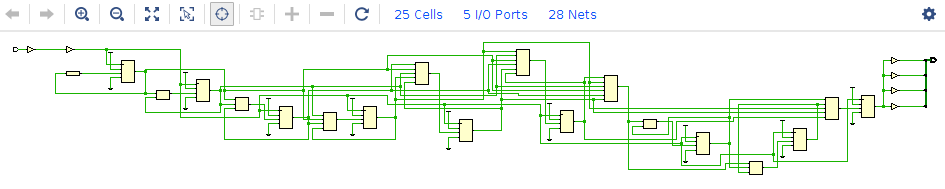
\includegraphics[width=10cm]{BDCLed_SYN.png}}
\caption{\label{fig:BDCLedSYN} BDCLed Synthesized Schematic; Xilinx Vivado 2017.4}
\end{figure}

    \begin{figure}
\centerline{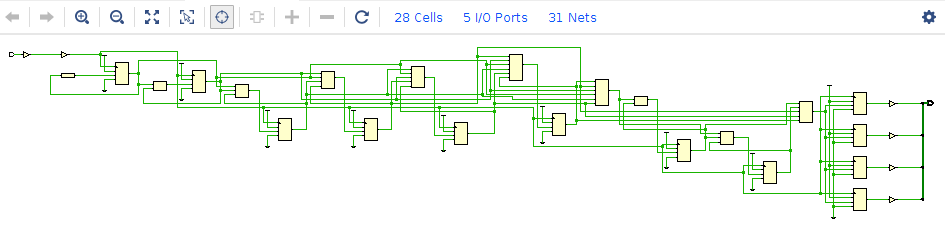
\includegraphics[width=10cm]{BDCLed_IMP.png}}
\caption{\label{fig:BDCLedSYN} BDCLed Implementated Schematic; Xilinx Vivado 2017.4}
\end{figure}

    \subsection{PYNQ-Z1 Constraints File}\label{pynq-z1-constraints-file}

uses the same constraint file \texttt{constrs\_countLED.xdc} as the
project \textbf{Project 3: Countdown}

    \subsection{Verilog Testbench}\label{verilog-testbench}

    \begin{Verbatim}[commandchars=\\\{\}]
{\color{incolor}In [{\color{incolor}31}]:} \PY{n+nd}{@block}
         \PY{k}{def} \PY{n+nf}{BDCLed\PYZus{}TBV}\PY{p}{(}\PY{p}{)}\PY{p}{:}
             \PY{l+s+sd}{\PYZdq{}\PYZdq{}\PYZdq{}}
         \PY{l+s+sd}{    myHDL \PYZhy{}\PYZgt{} Verilog Testbench for `BDCLed`}
         \PY{l+s+sd}{    \PYZdq{}\PYZdq{}\PYZdq{}}
         
             \PY{n}{clk}\PY{o}{=}\PY{n}{Signal}\PY{p}{(}\PY{n+nb}{bool}\PY{p}{(}\PY{l+m+mi}{0}\PY{p}{)}\PY{p}{)}
             \PY{n}{led}\PY{o}{=}\PY{n}{Signal}\PY{p}{(}\PY{n}{intbv}\PY{p}{(}\PY{l+m+mi}{0}\PY{p}{)}\PY{p}{[}\PY{l+m+mi}{4}\PY{p}{:}\PY{p}{]}\PY{p}{)}
             
             \PY{n+nd}{@always\PYZus{}comb}
             \PY{k}{def} \PY{n+nf}{print\PYZus{}data}\PY{p}{(}\PY{p}{)}\PY{p}{:}
                 \PY{n+nb}{print}\PY{p}{(}\PY{n}{sw}\PY{p}{,} \PY{n}{clk}\PY{p}{,} \PY{n}{led}\PY{p}{)}
         
             \PY{n}{DUT}\PY{o}{=}\PY{n}{BDCLed}\PY{p}{(}\PY{n}{clk}\PY{p}{,} \PY{n}{led}\PY{p}{)}
             
             
             \PY{n+nd}{@instance}
             \PY{k}{def} \PY{n+nf}{clk\PYZus{}signal}\PY{p}{(}\PY{p}{)}\PY{p}{:}
                 \PY{k}{while} \PY{k+kc}{True}\PY{p}{:}
                     \PY{n}{clk}\PY{o}{.}\PY{n}{next} \PY{o}{=} \PY{o+ow}{not} \PY{n}{clk}
                     \PY{k}{yield} \PY{n}{delay}\PY{p}{(}\PY{l+m+mi}{1}\PY{p}{)}
                 
             \PY{n+nd}{@instance}
             \PY{k}{def} \PY{n+nf}{stimules}\PY{p}{(}\PY{p}{)}\PY{p}{:}
                 \PY{n}{i}\PY{o}{=}\PY{l+m+mi}{0}
                 \PY{k}{while} \PY{k+kc}{True}\PY{p}{:}
                     \PY{k}{if} \PY{n}{i}\PY{o}{==}\PY{l+m+mi}{1000}\PY{p}{:}
                         \PY{k}{raise} \PY{n}{StopSimulation}\PY{p}{(}\PY{p}{)}
                     \PY{n}{i}\PY{o}{+}\PY{o}{=}\PY{l+m+mi}{1}
                     \PY{k}{yield} \PY{n}{clk}\PY{o}{.}\PY{n}{posedge}
             
             \PY{k}{return} \PY{n}{instances}\PY{p}{(}\PY{p}{)}
                     
         \PY{n}{TB}\PY{o}{=}\PY{n}{BDCLed\PYZus{}TBV}\PY{p}{(}\PY{p}{)}
         \PY{n}{TB}\PY{o}{.}\PY{n}{convert}\PY{p}{(}\PY{n}{hdl}\PY{o}{=}\PY{l+s+s2}{\PYZdq{}}\PY{l+s+s2}{Verilog}\PY{l+s+s2}{\PYZdq{}}\PY{p}{,} \PY{n}{initial\PYZus{}values}\PY{o}{=}\PY{k+kc}{True}\PY{p}{)}
         \PY{n}{VerilogTextReader}\PY{p}{(}\PY{l+s+s1}{\PYZsq{}}\PY{l+s+s1}{BDCLed\PYZus{}TBV}\PY{l+s+s1}{\PYZsq{}}\PY{p}{)}\PY{p}{;}
\end{Verbatim}


    \begin{Verbatim}[commandchars=\\\{\}]
<class 'myhdl.\_Signal.\_Signal'> <class '\_ast.Name'>
<class 'myhdl.\_Signal.\_Signal'> <class '\_ast.Name'>
<class 'myhdl.\_Signal.\_Signal'> <class '\_ast.Name'>
***Verilog modual from BDCLed\_TBV.v***

 // File: BDCLed\_TBV.v
// Generated by MyHDL 0.10
// Date: Mon Aug 20 11:02:51 2018


`timescale 1ns/10ps

module BDCLed\_TBV (

);
// myHDL -> Verilog Testbench for `BDCLed`


reg clk = 0;
wire [1:0] sw;
reg [3:0] led = 0;
wire [7:0] BDCLed0\_0\_duty\_led;
reg [7:0] BDCLed0\_0\_counter = 0;

assign sw = 2'd0;
assign BDCLed0\_0\_duty\_led = 8'd8;


always @(sw, led, clk) begin: BDCLED\_TBV\_PRINT\_DATA
    \$write("\%h", sw);
    \$write(" ");
    \$write("\%h", clk);
    \$write(" ");
    \$write("\%h", led);
    \$write("\textbackslash{}n");
end


always @(posedge clk) begin: BDCLED\_TBV\_BDCLED0\_0\_LOGIC
    BDCLed0\_0\_counter <= (BDCLed0\_0\_counter + 1);
    if ((BDCLed0\_0\_counter < BDCLed0\_0\_duty\_led)) begin
        led <= 15;
    end
    else begin
        led <= 0;
    end
end


initial begin: BDCLED\_TBV\_CLK\_SIGNAL
    while (1'b1) begin
        clk <= (!clk);
        \# 1;
    end
end


initial begin: BDCLED\_TBV\_STIMULES
    integer i;
    i = 0;
    while (1'b1) begin
        if ((i == 1000)) begin
            \$finish;
        end
        i = i + 1;
        @(posedge clk);
    end
end

endmodule


    \end{Verbatim}

    \begin{Verbatim}[commandchars=\\\{\}]
/home/iridium/anaconda3/lib/python3.6/site-packages/myhdl/conversion/\_toVerilog.py:349: ToVerilogWarning: Signal is not driven: sw
  category=ToVerilogWarning
/home/iridium/anaconda3/lib/python3.6/site-packages/myhdl/conversion/\_toVerilog.py:349: ToVerilogWarning: Signal is not driven: BDCLed0\_0\_duty\_led
  category=ToVerilogWarning

    \end{Verbatim}

    \subsection{Board Verification}\label{board-verification}

    \section{Project 5: Mid-level PWM
LED}\label{project-5-mid-level-pwm-led}

From https://timetoexplore.net/blog/arty-fpga-verilog-02 creates a
mildly complex Pulse Width Modulator (PWM) module to then be deployed in
a top module counter/assignment module to create various level PWM
brightness for each of the LEDs

    \subsubsection{PWM myHDL Code}\label{pwm-myhdl-code}

    \begin{Verbatim}[commandchars=\\\{\}]
{\color{incolor}In [{\color{incolor}33}]:} \PY{n+nd}{@block}
         \PY{k}{def} \PY{n+nf}{PWM}\PY{p}{(}\PY{n}{clk}\PY{p}{,} \PY{n}{dutyCount}\PY{p}{,} \PY{n}{ofState}\PY{p}{)}\PY{p}{:}
             \PY{l+s+sd}{\PYZdq{}\PYZdq{}\PYZdq{}}
         \PY{l+s+sd}{    pwm module}
         \PY{l+s+sd}{    }
         \PY{l+s+sd}{    Inputs:}
         \PY{l+s+sd}{        clk(bool): clock}
         \PY{l+s+sd}{        dutyCount(bitVec): clock cycle percent on time value}
         \PY{l+s+sd}{        using an 8Bit internal counter}
         \PY{l+s+sd}{        }
         \PY{l+s+sd}{    Ouputs:}
         \PY{l+s+sd}{        ofState(bool): on/off state signal of the PWM}
         \PY{l+s+sd}{    }
         \PY{l+s+sd}{    \PYZdq{}\PYZdq{}\PYZdq{}}
             \PY{n}{counter}\PY{o}{=}\PY{n}{Signal}\PY{p}{(}\PY{n}{modbv}\PY{p}{(}\PY{l+m+mi}{0}\PY{p}{)}\PY{p}{[}\PY{l+m+mi}{8}\PY{p}{:}\PY{p}{]}\PY{p}{)}
             
             \PY{n+nd}{@always}\PY{p}{(}\PY{n}{clk}\PY{o}{.}\PY{n}{posedge}\PY{p}{)}
             \PY{k}{def} \PY{n+nf}{logic}\PY{p}{(}\PY{p}{)}\PY{p}{:}
                 \PY{n}{counter}\PY{o}{.}\PY{n}{next}\PY{o}{=}\PY{n}{counter}\PY{o}{+}\PY{l+m+mi}{1}
                 \PY{n}{ofState}\PY{o}{.}\PY{n}{next}\PY{o}{=}\PY{n}{counter}\PY{o}{\PYZlt{}}\PY{n}{dutyCount}
             
             \PY{k}{return} \PY{n}{instances}\PY{p}{(}\PY{p}{)}
\end{Verbatim}


    \subsubsection{PWM myHDL Testing}\label{pwm-myhdl-testing}

    \begin{Verbatim}[commandchars=\\\{\}]
{\color{incolor}In [{\color{incolor}35}]:} \PY{n}{Peeker}\PY{o}{.}\PY{n}{clear}\PY{p}{(}\PY{p}{)}
         
         \PY{n}{clk}\PY{o}{=}\PY{n}{Signal}\PY{p}{(}\PY{n+nb}{bool}\PY{p}{(}\PY{l+m+mi}{0}\PY{p}{)}\PY{p}{)}\PY{p}{;} \PY{n}{Peeker}\PY{p}{(}\PY{n}{clk}\PY{p}{,} \PY{l+s+s1}{\PYZsq{}}\PY{l+s+s1}{clk}\PY{l+s+s1}{\PYZsq{}}\PY{p}{)}
         \PY{n}{dutyCount}\PY{o}{=}\PY{n}{Signal}\PY{p}{(}\PY{n}{intbv}\PY{p}{(}\PY{l+m+mi}{0}\PY{p}{)}\PY{p}{[}\PY{l+m+mi}{8}\PY{p}{:}\PY{p}{]}\PY{p}{)}\PY{p}{;} \PY{n}{Peeker}\PY{p}{(}\PY{n}{dutyCount}\PY{p}{,} \PY{l+s+s1}{\PYZsq{}}\PY{l+s+s1}{dutyCount}\PY{l+s+s1}{\PYZsq{}}\PY{p}{)}
         \PY{n}{ofState}\PY{o}{=}\PY{n}{Signal}\PY{p}{(}\PY{n+nb}{bool}\PY{p}{(}\PY{l+m+mi}{0}\PY{p}{)}\PY{p}{)}\PY{p}{;} \PY{n}{Peeker}\PY{p}{(}\PY{n}{ofState}\PY{p}{,} \PY{l+s+s1}{\PYZsq{}}\PY{l+s+s1}{ofState}\PY{l+s+s1}{\PYZsq{}}\PY{p}{)}
         
         \PY{n}{DUT}\PY{o}{=}\PY{n}{PWM}\PY{p}{(}\PY{n}{clk}\PY{p}{,} \PY{n}{dutyCount}\PY{p}{,} \PY{n}{ofState}\PY{p}{)}
         
         \PY{k}{def} \PY{n+nf}{PWM\PYZus{}TB}\PY{p}{(}\PY{p}{)}\PY{p}{:}
             \PY{l+s+sd}{\PYZdq{}\PYZdq{}\PYZdq{}}
         \PY{l+s+sd}{    myHDL only Testbench for `PWM`}
         \PY{l+s+sd}{    \PYZdq{}\PYZdq{}\PYZdq{}}
             
             \PY{n+nd}{@always}\PY{p}{(}\PY{n}{delay}\PY{p}{(}\PY{l+m+mi}{1}\PY{p}{)}\PY{p}{)}
             \PY{k}{def} \PY{n+nf}{ClkGen}\PY{p}{(}\PY{p}{)}\PY{p}{:}
                 \PY{n}{clk}\PY{o}{.}\PY{n}{next}\PY{o}{=}\PY{o+ow}{not} \PY{n}{clk}
                 
             \PY{n+nd}{@instance}
             \PY{k}{def} \PY{n+nf}{stimules}\PY{p}{(}\PY{p}{)}\PY{p}{:}
                 \PY{n}{i}\PY{o}{=}\PY{l+m+mi}{0}
                 \PY{k}{while} \PY{k+kc}{True}\PY{p}{:}
                     \PY{k}{if} \PY{n}{i}\PY{o}{==}\PY{l+m+mi}{5}\PY{p}{:}
                         \PY{n}{dutyCount}\PY{o}{.}\PY{n}{next}\PY{o}{=}\PY{l+m+mi}{20}
                     \PY{k}{elif} \PY{n}{i}\PY{o}{==}\PY{l+m+mi}{45}\PY{p}{:}
                         \PY{n}{dutyCount}\PY{o}{.}\PY{n}{next}\PY{o}{=}\PY{l+m+mi}{80}
                     \PY{k}{elif} \PY{n}{i}\PY{o}{==}\PY{l+m+mi}{100}\PY{p}{:}
                         \PY{k}{raise} \PY{n}{StopSimulation}\PY{p}{(}\PY{p}{)}
                     \PY{n}{i}\PY{o}{+}\PY{o}{=}\PY{l+m+mi}{1}
                     \PY{k}{yield} \PY{n}{clk}\PY{o}{.}\PY{n}{posedge}
             
             \PY{k}{return} \PY{n}{instances}\PY{p}{(}\PY{p}{)}
         
         \PY{n}{sim}\PY{o}{=}\PY{n}{Simulation}\PY{p}{(}\PY{n}{DUT}\PY{p}{,} \PY{n}{PWM\PYZus{}TB}\PY{p}{(}\PY{p}{)}\PY{p}{,} \PY{o}{*}\PY{n}{Peeker}\PY{o}{.}\PY{n}{instances}\PY{p}{(}\PY{p}{)}\PY{p}{)}\PY{o}{.}\PY{n}{run}\PY{p}{(}\PY{p}{)}
\end{Verbatim}


    \begin{Verbatim}[commandchars=\\\{\}]
{\color{incolor}In [{\color{incolor}36}]:} \PY{n}{Peeker}\PY{o}{.}\PY{n}{to\PYZus{}wavedrom}\PY{p}{(}\PY{p}{)}
\end{Verbatim}


    
    
    
    
    \begin{Verbatim}[commandchars=\\\{\}]
{\color{incolor}In [{\color{incolor} }]:} \PY{n}{pwmData}\PY{o}{=}\PY{n}{Peeker}\PY{o}{.}\PY{n}{to\PYZus{}dataframe}\PY{p}{(}\PY{p}{)}
        \PY{n}{pwmData}\PY{o}{=}\PY{n}{pwmData}\PY{p}{[}\PY{n}{pwmData}\PY{p}{[}\PY{l+s+s1}{\PYZsq{}}\PY{l+s+s1}{clk}\PY{l+s+s1}{\PYZsq{}}\PY{p}{]}\PY{o}{==}\PY{l+m+mi}{1}\PY{p}{]}
        \PY{n}{pwmData}\PY{o}{.}\PY{n}{reset\PYZus{}index}\PY{p}{(}\PY{n}{drop}\PY{o}{=}\PY{k+kc}{True}\PY{p}{,} \PY{n}{inplace}\PY{o}{=}\PY{k+kc}{True}\PY{p}{)}
        \PY{n}{pwmData}\PY{o}{.}\PY{n}{plot}\PY{p}{(}\PY{n}{y}\PY{o}{=}\PY{p}{[}\PY{l+s+s1}{\PYZsq{}}\PY{l+s+s1}{dutyCount}\PY{l+s+s1}{\PYZsq{}}\PY{p}{,} \PY{l+s+s1}{\PYZsq{}}\PY{l+s+s1}{ofState}\PY{l+s+s1}{\PYZsq{}}\PY{p}{]}\PY{p}{)}\PY{p}{;}
\end{Verbatim}


    \subsection{pwm Verilog Code}\label{pwm-verilog-code}

    \begin{Verbatim}[commandchars=\\\{\}]
{\color{incolor}In [{\color{incolor} }]:} \PY{n}{DUT}\PY{o}{.}\PY{n}{convert}\PY{p}{(}\PY{p}{)}
        \PY{n}{VerilogTextReader}\PY{p}{(}\PY{l+s+s1}{\PYZsq{}}\PY{l+s+s1}{pwm}\PY{l+s+s1}{\PYZsq{}}\PY{p}{)}\PY{p}{;}
\end{Verbatim}


    \begin{figure}
\centerline{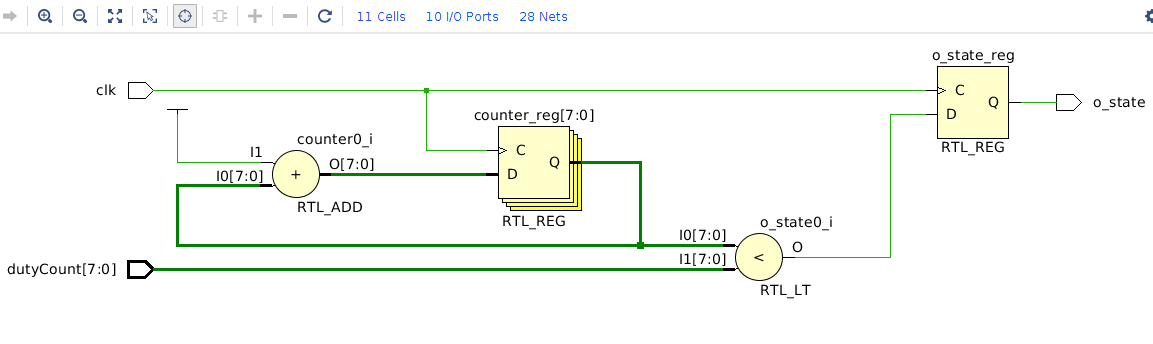
\includegraphics[width=10cm]{pwm_RTL.png}}
\caption{\label{fig:pwmRTL} pwm RTL schematic; Xilinx Vivado 2017.4}
\end{figure}

    \begin{figure}
\centerline{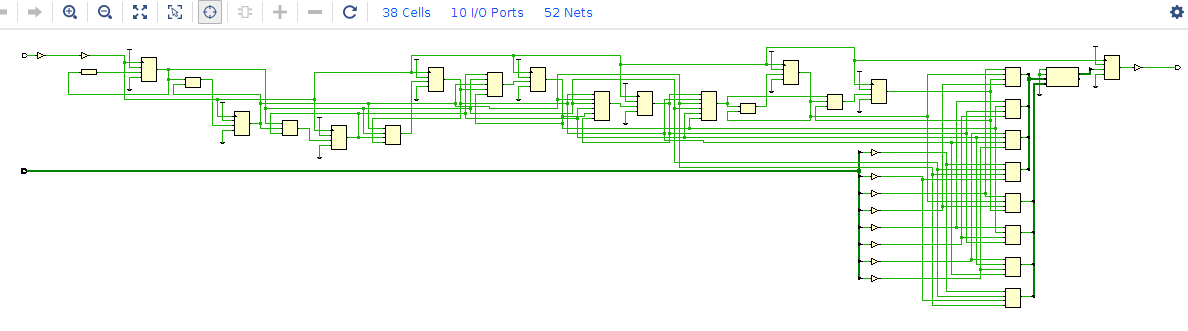
\includegraphics[width=10cm]{pwm_SYN.png}}
\caption{\label{fig:pwmSYN} pwm Synthesized Schematic; Xilinx Vivado 2017.4}
\end{figure}

    \subsection{pwm PYNQ-Z1 Constraints
File}\label{pwm-pynq-z1-constraints-file}

this module is a sup module and therefore was not taken beyond synthisis
and thus has no contraint file

    \subsection{pwm Verilog Testbench}\label{pwm-verilog-testbench}

    \begin{Verbatim}[commandchars=\\\{\}]
{\color{incolor}In [{\color{incolor} }]:} \PY{n+nd}{@block}
        \PY{k}{def} \PY{n+nf}{pwm\PYZus{}TBV}\PY{p}{(}\PY{p}{)}\PY{p}{:}
        
            \PY{n}{clk}\PY{o}{=}\PY{n}{Signal}\PY{p}{(}\PY{n+nb}{bool}\PY{p}{(}\PY{l+m+mi}{0}\PY{p}{)}\PY{p}{)}
            \PY{n}{dutyCount}\PY{o}{=}\PY{n}{Signal}\PY{p}{(}\PY{n}{intbv}\PY{p}{(}\PY{l+m+mi}{0}\PY{p}{)}\PY{p}{[}\PY{l+m+mi}{8}\PY{p}{:}\PY{p}{]}\PY{p}{)}
            \PY{n}{ofState}\PY{o}{=}\PY{n}{Signal}\PY{p}{(}\PY{n+nb}{bool}\PY{p}{(}\PY{l+m+mi}{0}\PY{p}{)}\PY{p}{)}
            
            \PY{n+nd}{@always\PYZus{}comb}
            \PY{k}{def} \PY{n+nf}{print\PYZus{}data}\PY{p}{(}\PY{p}{)}\PY{p}{:}
                \PY{n+nb}{print}\PY{p}{(}\PY{n}{clk}\PY{p}{,} \PY{n}{dutyCount}\PY{p}{,} \PY{n}{ofState}\PY{p}{)}
        
            \PY{n}{DUT}\PY{o}{=}\PY{n}{pwm}\PY{p}{(}\PY{n}{clk}\PY{p}{,} \PY{n}{dutyCount}\PY{p}{,} \PY{n}{ofState}\PY{p}{)}
            
            \PY{n+nd}{@instance}
            \PY{k}{def} \PY{n+nf}{clk\PYZus{}signal}\PY{p}{(}\PY{p}{)}\PY{p}{:}
                \PY{k}{while} \PY{k+kc}{True}\PY{p}{:}
                    \PY{n}{clk}\PY{o}{.}\PY{n}{next} \PY{o}{=} \PY{o+ow}{not} \PY{n}{clk}
                    \PY{k}{yield} \PY{n}{delay}\PY{p}{(}\PY{l+m+mi}{1}\PY{p}{)}
                
            \PY{n+nd}{@instance}
            \PY{k}{def} \PY{n+nf}{stimules}\PY{p}{(}\PY{p}{)}\PY{p}{:}
                \PY{n}{i}\PY{o}{=}\PY{l+m+mi}{0}
                \PY{k}{while} \PY{k+kc}{True}\PY{p}{:}
                    \PY{k}{if} \PY{n}{i}\PY{o}{==}\PY{l+m+mi}{5}\PY{p}{:}
                        \PY{n}{dutyCount}\PY{o}{.}\PY{n}{next}\PY{o}{=}\PY{l+m+mi}{20}
                    \PY{k}{elif} \PY{n}{i}\PY{o}{==}\PY{l+m+mi}{45}\PY{p}{:}
                        \PY{n}{dutyCount}\PY{o}{.}\PY{n}{next}\PY{o}{=}\PY{l+m+mi}{80}
                    \PY{k}{elif} \PY{n}{i}\PY{o}{==}\PY{l+m+mi}{100}\PY{p}{:}
                        \PY{k}{raise} \PY{n}{StopSimulation}\PY{p}{(}\PY{p}{)}
                    \PY{k}{else}\PY{p}{:}
                        \PY{k}{pass}
                    \PY{n}{i}\PY{o}{+}\PY{o}{=}\PY{l+m+mi}{1}
                    \PY{k}{yield} \PY{n}{clk}\PY{o}{.}\PY{n}{posedge}
            
            \PY{k}{return} \PY{n}{instances}\PY{p}{(}\PY{p}{)}
        
        \PY{n}{TB}\PY{o}{=}\PY{n}{pwm\PYZus{}TBV}\PY{p}{(}\PY{p}{)}
        \PY{n}{TB}\PY{o}{.}\PY{n}{convert}\PY{p}{(}\PY{n}{hdl}\PY{o}{=}\PY{l+s+s2}{\PYZdq{}}\PY{l+s+s2}{Verilog}\PY{l+s+s2}{\PYZdq{}}\PY{p}{,} \PY{n}{initial\PYZus{}values}\PY{o}{=}\PY{k+kc}{True}\PY{p}{)}
        \PY{n}{VerilogTextReader}\PY{p}{(}\PY{l+s+s1}{\PYZsq{}}\PY{l+s+s1}{countLED\PYZus{}TBV}\PY{l+s+s1}{\PYZsq{}}\PY{p}{)}\PY{p}{;}
\end{Verbatim}


    \subsection{top myHDL Code}\label{top-myhdl-code}

    \begin{Verbatim}[commandchars=\\\{\}]
{\color{incolor}In [{\color{incolor} }]:} \PY{n+nd}{@block}
        \PY{k}{def} \PY{n+nf}{top}\PY{p}{(}\PY{n}{clk}\PY{p}{,} \PY{n}{led}\PY{p}{)}\PY{p}{:}
            \PY{n}{led\PYZus{}i}\PY{o}{=}\PY{p}{[}\PY{n}{Signal}\PY{p}{(}\PY{n+nb}{bool}\PY{p}{(}\PY{l+m+mi}{0}\PY{p}{)}\PY{p}{)} \PY{k}{for} \PY{n}{\PYZus{}} \PY{o+ow}{in} \PY{n+nb}{range}\PY{p}{(}\PY{l+m+mi}{4}\PY{p}{)}\PY{p}{]}
            \PY{n}{pwmled0}\PY{o}{=}\PY{n}{pwm}\PY{p}{(}\PY{n}{clk}\PY{o}{=}\PY{n}{clk}\PY{p}{,} \PY{n}{dutyCount}\PY{o}{=}\PY{n}{Signal}\PY{p}{(}\PY{n}{intbv}\PY{p}{(}\PY{l+m+mi}{4}\PY{p}{)}\PY{p}{[}\PY{l+m+mi}{8}\PY{p}{:}\PY{p}{]}\PY{p}{)}\PY{p}{,} \PY{n}{ofState}\PY{o}{=}\PY{n}{led\PYZus{}i}\PY{p}{[}\PY{l+m+mi}{0}\PY{p}{]}\PY{p}{)}
            \PY{n}{pwmled1}\PY{o}{=}\PY{n}{pwm}\PY{p}{(}\PY{n}{clk}\PY{o}{=}\PY{n}{clk}\PY{p}{,} \PY{n}{dutyCount}\PY{o}{=}\PY{n}{Signal}\PY{p}{(}\PY{n}{intbv}\PY{p}{(}\PY{l+m+mi}{16}\PY{p}{)}\PY{p}{[}\PY{l+m+mi}{8}\PY{p}{:}\PY{p}{]}\PY{p}{)}\PY{p}{,} \PY{n}{ofState}\PY{o}{=}\PY{n}{led\PYZus{}i}\PY{p}{[}\PY{l+m+mi}{1}\PY{p}{]}\PY{p}{)}
            \PY{n}{pwmled2}\PY{o}{=}\PY{n}{pwm}\PY{p}{(}\PY{n}{clk}\PY{o}{=}\PY{n}{clk}\PY{p}{,} \PY{n}{dutyCount}\PY{o}{=}\PY{n}{Signal}\PY{p}{(}\PY{n}{intbv}\PY{p}{(}\PY{l+m+mi}{64}\PY{p}{)}\PY{p}{[}\PY{l+m+mi}{8}\PY{p}{:}\PY{p}{]}\PY{p}{)}\PY{p}{,} \PY{n}{ofState}\PY{o}{=}\PY{n}{led\PYZus{}i}\PY{p}{[}\PY{l+m+mi}{2}\PY{p}{]}\PY{p}{)}
            \PY{n}{pwmled3}\PY{o}{=}\PY{n}{pwm}\PY{p}{(}\PY{n}{clk}\PY{o}{=}\PY{n}{clk}\PY{p}{,} \PY{n}{dutyCount}\PY{o}{=}\PY{n}{Signal}\PY{p}{(}\PY{n}{intbv}\PY{p}{(}\PY{l+m+mi}{255}\PY{p}{)}\PY{p}{[}\PY{l+m+mi}{8}\PY{p}{:}\PY{p}{]}\PY{p}{)}\PY{p}{,} \PY{n}{ofState}\PY{o}{=}\PY{n}{led\PYZus{}i}\PY{p}{[}\PY{l+m+mi}{3}\PY{p}{]}\PY{p}{)}
            
            \PY{n+nd}{@always\PYZus{}comb}
            \PY{k}{def} \PY{n+nf}{ouputBuffer}\PY{p}{(}\PY{p}{)}\PY{p}{:}
                \PY{n}{led}\PY{o}{.}\PY{n}{next}\PY{o}{=}\PY{n}{concat}\PY{p}{(}\PY{n}{led\PYZus{}i}\PY{p}{[}\PY{l+m+mi}{3}\PY{p}{]}\PY{p}{,} \PY{n}{led\PYZus{}i}\PY{p}{[}\PY{l+m+mi}{2}\PY{p}{]}\PY{p}{,} \PY{n}{led\PYZus{}i}\PY{p}{[}\PY{l+m+mi}{1}\PY{p}{]}\PY{p}{,} \PY{n}{led\PYZus{}i}\PY{p}{[}\PY{l+m+mi}{0}\PY{p}{]}\PY{p}{)}
            \PY{k}{return} \PY{n}{instances}\PY{p}{(}\PY{p}{)}
\end{Verbatim}


    \begin{Verbatim}[commandchars=\\\{\}]
{\color{incolor}In [{\color{incolor} }]:} \PY{n}{Peeker}\PY{o}{.}\PY{n}{clear}\PY{p}{(}\PY{p}{)}
        \PY{n}{clk}\PY{o}{=}\PY{n}{Signal}\PY{p}{(}\PY{n+nb}{bool}\PY{p}{(}\PY{l+m+mi}{0}\PY{p}{)}\PY{p}{)}\PY{p}{;} \PY{n}{Peeker}\PY{p}{(}\PY{n}{clk}\PY{p}{,} \PY{l+s+s1}{\PYZsq{}}\PY{l+s+s1}{clk}\PY{l+s+s1}{\PYZsq{}}\PY{p}{)}
        \PY{n}{led}\PY{o}{=}\PY{n}{Signal}\PY{p}{(}\PY{n}{intbv}\PY{p}{(}\PY{l+m+mi}{0}\PY{p}{)}\PY{p}{[}\PY{l+m+mi}{4}\PY{p}{:}\PY{p}{]}\PY{p}{)}\PY{p}{;} \PY{n}{Peeker}\PY{p}{(}\PY{n}{led}\PY{p}{,} \PY{l+s+s1}{\PYZsq{}}\PY{l+s+s1}{led}\PY{l+s+s1}{\PYZsq{}}\PY{p}{)}
        
        \PY{n}{DUT}\PY{o}{=}\PY{n}{top}\PY{p}{(}\PY{n}{clk}\PY{p}{,} \PY{n}{led}\PY{p}{)}
        
        
        \PY{k}{def} \PY{n+nf}{top\PYZus{}TB}\PY{p}{(}\PY{p}{)}\PY{p}{:}
            \PY{n+nd}{@always}\PY{p}{(}\PY{n}{delay}\PY{p}{(}\PY{l+m+mi}{1}\PY{p}{)}\PY{p}{)}
            \PY{k}{def} \PY{n+nf}{ClkGen}\PY{p}{(}\PY{p}{)}\PY{p}{:}
                \PY{n}{clk}\PY{o}{.}\PY{n}{next}\PY{o}{=}\PY{o+ow}{not} \PY{n}{clk}
                
            \PY{n+nd}{@instance}
            \PY{k}{def} \PY{n+nf}{stimules}\PY{p}{(}\PY{p}{)}\PY{p}{:}
                \PY{n}{i}\PY{o}{=}\PY{l+m+mi}{0}
                \PY{k}{while} \PY{k+kc}{True}\PY{p}{:}
                    \PY{k}{if} \PY{n}{i}\PY{o}{==}\PY{l+m+mi}{1000}\PY{p}{:}
                        \PY{k}{raise} \PY{n}{StopSimulation}\PY{p}{(}\PY{p}{)}
                    \PY{n}{i}\PY{o}{+}\PY{o}{=}\PY{l+m+mi}{1}
                    \PY{k}{yield} \PY{n}{clk}\PY{o}{.}\PY{n}{posedge}
            
            \PY{k}{return} \PY{n}{instances}\PY{p}{(}\PY{p}{)}
        
        \PY{n}{sim}\PY{o}{=}\PY{n}{Simulation}\PY{p}{(}\PY{n}{DUT}\PY{p}{,} \PY{n}{top\PYZus{}TB}\PY{p}{(}\PY{p}{)}\PY{p}{,} \PY{o}{*}\PY{n}{Peeker}\PY{o}{.}\PY{n}{instances}\PY{p}{(}\PY{p}{)}\PY{p}{)}\PY{o}{.}\PY{n}{run}\PY{p}{(}\PY{p}{)}
\end{Verbatim}


    \begin{Verbatim}[commandchars=\\\{\}]
{\color{incolor}In [{\color{incolor} }]:} \PY{n}{Peeker}\PY{o}{.}\PY{n}{to\PYZus{}wavedrom}\PY{p}{(}\PY{p}{)}
\end{Verbatim}


    \begin{Verbatim}[commandchars=\\\{\}]
{\color{incolor}In [{\color{incolor} }]:} \PY{n}{topData}\PY{o}{=}\PY{n}{Peeker}\PY{o}{.}\PY{n}{to\PYZus{}dataframe}\PY{p}{(}\PY{p}{)}
        \PY{n}{topData}\PY{o}{=}\PY{n}{topData}\PY{p}{[}\PY{n}{topData}\PY{p}{[}\PY{l+s+s1}{\PYZsq{}}\PY{l+s+s1}{clk}\PY{l+s+s1}{\PYZsq{}}\PY{p}{]}\PY{o}{==}\PY{l+m+mi}{1}\PY{p}{]}
        \PY{n}{topData}\PY{o}{.}\PY{n}{reset\PYZus{}index}\PY{p}{(}\PY{n}{drop}\PY{o}{=}\PY{k+kc}{True}\PY{p}{,} \PY{n}{inplace}\PY{o}{=}\PY{k+kc}{True}\PY{p}{)}
        \PY{n}{topData}\PY{o}{.}\PY{n}{plot}\PY{p}{(}\PY{n}{y}\PY{o}{=}\PY{l+s+s1}{\PYZsq{}}\PY{l+s+s1}{led}\PY{l+s+s1}{\PYZsq{}}\PY{p}{)}
\end{Verbatim}


    \begin{Verbatim}[commandchars=\\\{\}]
{\color{incolor}In [{\color{incolor} }]:} \PY{n}{DUT}\PY{o}{.}\PY{n}{convert}\PY{p}{(}\PY{p}{)}
        \PY{n}{VerilogTextReader}\PY{p}{(}\PY{l+s+s1}{\PYZsq{}}\PY{l+s+s1}{top}\PY{l+s+s1}{\PYZsq{}}\PY{p}{)}\PY{p}{;}
\end{Verbatim}


    \begin{Verbatim}[commandchars=\\\{\}]
{\color{incolor}In [{\color{incolor} }]:} \PY{n+nd}{@block}
        \PY{k}{def} \PY{n+nf}{top\PYZus{}TBV}\PY{p}{(}\PY{p}{)}\PY{p}{:}
        
            \PY{n}{clk}\PY{o}{=}\PY{n}{Signal}\PY{p}{(}\PY{n+nb}{bool}\PY{p}{(}\PY{l+m+mi}{0}\PY{p}{)}\PY{p}{)}
            \PY{n}{led}\PY{o}{=}\PY{n}{Signal}\PY{p}{(}\PY{n}{intbv}\PY{p}{(}\PY{l+m+mi}{0}\PY{p}{)}\PY{p}{[}\PY{l+m+mi}{4}\PY{p}{:}\PY{p}{]}\PY{p}{)}
            
            \PY{n+nd}{@always\PYZus{}comb}
            \PY{k}{def} \PY{n+nf}{print\PYZus{}data}\PY{p}{(}\PY{p}{)}\PY{p}{:}
                \PY{n+nb}{print}\PY{p}{(}\PY{n}{clk}\PY{p}{,} \PY{n}{led}\PY{p}{)}
        
            \PY{n}{DUT}\PY{o}{=}\PY{n}{top}\PY{p}{(}\PY{n}{clk}\PY{p}{,} \PY{n}{led}\PY{p}{)}
            
            \PY{n+nd}{@instance}
            \PY{k}{def} \PY{n+nf}{clk\PYZus{}signal}\PY{p}{(}\PY{p}{)}\PY{p}{:}
                \PY{k}{while} \PY{k+kc}{True}\PY{p}{:}
                    \PY{n}{clk}\PY{o}{.}\PY{n}{next} \PY{o}{=} \PY{o+ow}{not} \PY{n}{clk}
                    \PY{k}{yield} \PY{n}{delay}\PY{p}{(}\PY{l+m+mi}{1}\PY{p}{)}
                
            \PY{n+nd}{@instance}
            \PY{k}{def} \PY{n+nf}{stimules}\PY{p}{(}\PY{p}{)}\PY{p}{:}
                \PY{n}{i}\PY{o}{=}\PY{l+m+mi}{0}
                \PY{k}{while} \PY{k+kc}{True}\PY{p}{:}
                    \PY{k}{if} \PY{n}{i}\PY{o}{==}\PY{l+m+mi}{1000}\PY{p}{:}
                        \PY{k}{raise} \PY{n}{StopSimulation}\PY{p}{(}\PY{p}{)}
                    
                    \PY{n}{i}\PY{o}{+}\PY{o}{=}\PY{l+m+mi}{1}
                    \PY{k}{yield} \PY{n}{clk}\PY{o}{.}\PY{n}{posedge}
            
            \PY{k}{return} \PY{n}{instances}\PY{p}{(}\PY{p}{)}
        
        \PY{n}{TB}\PY{o}{=}\PY{n}{top\PYZus{}TBV}\PY{p}{(}\PY{p}{)}
        \PY{n}{TB}\PY{o}{.}\PY{n}{convert}\PY{p}{(}\PY{n}{hdl}\PY{o}{=}\PY{l+s+s2}{\PYZdq{}}\PY{l+s+s2}{Verilog}\PY{l+s+s2}{\PYZdq{}}\PY{p}{,} \PY{n}{initial\PYZus{}values}\PY{o}{=}\PY{k+kc}{True}\PY{p}{)}
        \PY{n}{VerilogTextReader}\PY{p}{(}\PY{l+s+s1}{\PYZsq{}}\PY{l+s+s1}{top\PYZus{}TBV}\PY{l+s+s1}{\PYZsq{}}\PY{p}{)}\PY{p}{;}
\end{Verbatim}



    % Add a bibliography block to the postdoc
    
    
    
    \end{document}
